\chapter{Improved Linear Source Formulation for Multi-physics and 2D/1D Applications}{
  \label{ch:Improved Linear Source Formulation for Multi-physics and 2D/1D Applications}
  %%% Multi-group Energy quantities %%%
\DeclareDocumentCommand{\gprime}{}{g^{\prime}}
% Cross-sections
\DeclareDocumentCommand{\xs}{ O{t} O{\loc} O{g}}{\ensuremath{\CrossSection_{#1}^{#3}(#2)}}
\DeclareDocumentCommand{\xst}{ O{\loc} O{g} }{\xs[t][#1][#2]}
\DeclareDocumentCommand{\xsa}{ O{\loc} O{g} }{\xs[a][#1][#2]}
\DeclareDocumentCommand{\xsf}{ O{\loc} O{\gprime} }{\xs[f][#1][#2]}
\DeclareDocumentCommand{\xss}{ o O{\loc} O{\dirprime\vdot\dir} O{\gprime \to g} }{
    \IfNoValueOrEmptyTF{#1}
    {\xs[s][#2,#3][#4]}
    {\xs[s,#1][#2][#4]}
}
\DeclareDocumentCommand{\spect}{ O{\loc} O{g} }{\ensuremath{\Spectrum^{#2}(#1)}}
\DeclareDocumentCommand{\nufis}{ O{\loc} O{\gprime} }{ \ensuremath{\nu\xsf[#1][#2]}}
\DeclareDocumentCommand{\D}{ O{\loc} O{g} }{\ensuremath{D^{#2}(#1)}}

% Flux
\DeclareDocumentCommand{\aflux}{ O{\loc} O{\dir} O{g} }{\ensuremath{\AngularFlux^{#3}(#1,#2)}}
\DeclareDocumentCommand{\sflux}{ O{\loc} O{\gprime} }{\ensuremath{\ScalarFlux^{#2}(#1)}}
\DeclareDocumentCommand{\current}{ O{\loc} O{g} }{\ensuremath{\Current^{#2}(#1)}}
\DeclareDocumentCommand{\fluxmoma}{ O{\ell} O{n} O{\loc} O{g} }{\ensuremath{\ScalarFlux^{#2,#4}_{#1}(#3)}}

% Source
\DeclareDocumentCommand{\source}{ O{\loc} O{\dir} O{g} }{\ensuremath{q^{#3}(#1,#2)}}
\DeclareDocumentCommand{\sourcemoma}{ O{\ell} O{n} O{\loc} O{g} }{\ensuremath{q^{#2,#4}_{#1}(#3)}}

  %%% Discrete Ordinates Quantities %%%
\DeclareDocumentCommand{\mprime}{}{m^{\prime}}
\DeclareDocumentCommand{\dirm}{ O{m} }{\dir_{#1}}
\DeclareDocumentCommand{\wt}{ O{m} }{\Weight_{#1}}

% Quadrature set
\DeclareDocumentCommand{\angquad}{ O{N} }{ \mathcal{M}_{#1} }

% Cross-Sections
\DeclareDocumentCommand{\xss}{ o O{\loc} O{ m^{\prime}\!\to m} O{\gprime\!\to g} }{
    \IfNoValueOrEmptyTF{#1}
    {\xs[s,#3][#2][#4]}
    {\xs[s,#1][#2][#4]}
}

% Flux
\DeclareDocumentCommand{\aflux}{ O{\loc} O{m} O{g}}{\ensuremath{\AngularFlux^{#3}_{#2}\!\left(#1\right)}}

% Source
\DeclareDocumentCommand{\source}{ O{\loc} O{m} O{g} }{\ensuremath{q^{#3}_{#2}\!\left(#1\right)}}

  %%% MOC quantities %%%
% Geometric
\DeclareDocumentCommand{\Length}{}{s}
\DeclareDocumentCommand{\NormalizedLength}{}{t}
\DeclareDocumentCommand{\len}{ O{} }{\Length_{#1}}
\DeclareDocumentCommand{\segl}{ O{mki} }{\Length_{#1}}
\DeclareDocumentCommand{\nlen}{ O{m} }{\NormalizedLength_{#1}}
\DeclareDocumentCommand{\nsegl}{ O{mki} }{\NormalizedLength_{#1}}

\DeclareDocumentCommand{\centroid}{ O{\loc} O{i} }{#1_{#2}^{\text{c}}}
\DeclareDocumentCommand{\locIn}{ O{\loc} O{mki} }{{#1}_{#2}^{\text{in}}}
\DeclareDocumentCommand{\locOut}{ O{\loc} O{mki} }{{#1}_{#2}^{\text{out}}}
\DeclareDocumentCommand{\locCent}{ O{\loc} O{mki} }{{#1}_{#2}^{\text{c}}}
\DeclareDocumentCommand{\M}{ o O{i}}{%
    \IfNoValueOrEmptyTF{#1}
        {\vec{M}_{#2}}
        {M_{#2,#1}}
}
\DeclareDocumentCommand{\C}{o O{i} O{g}}{%
    \IfNoValueOrEmptyTF{#1}
        {\vec{C}_{#2}^{#3}}
        {C_{#2,#1}^{#3}}
}


% Integration
\DeclareAutoPairedDelimiter{\MOCTrackIntegral}{\langle}{\rangle_{mki}}
\DeclareAutoPairedDelimiter{\MOCSingleAngleIntegral}{\langle}{\rangle_{mi}}
\DeclareAutoPairedDelimiter{\MOCIntegral}{\langle}{\rangle_{i}}

% Cross-sections
\DeclareDocumentCommand{\xs}{ O{t} O{i} O{g}}{\ensuremath{\CrossSection_{#1,#2}^{#3}}}
\DeclareDocumentCommand{\xst}{ O{i} O{g} }{\xs[t][#1][#2]}
\DeclareDocumentCommand{\xsa}{ O{i} O{g} }{\xs[a][#1][#2]}
\DeclareDocumentCommand{\xsf}{ O{i} O{\gprime} }{\xs[f][#1][#2]}
\DeclareDocumentCommand{\xss}{ o O{i} O{m'\to m} O{\gprime \to g} }{
    \IfNoValueOrEmptyTF{#1}
    {\xs[s][#2,#3][#4]}
    {\xs[s,#1][#2][#4]}
}

\DeclareDocumentCommand{\spect}{ O{i} O{g} }{\ensuremath{\Spectrum^{#2}_{#1}}}
\DeclareDocumentCommand{\nufis}{ O{i} O{\gprime} }{ \ensuremath{\nu\xsf[#1][#2]}}
\DeclareDocumentCommand{\D}{ O{i} O{g} }{\ensuremath{D^{#2}_{#1}}}
\DeclareDocumentCommand{\opt}{ O{m} O{g} }{\OpticalThickness_{#1}^{#2}}
\DeclareDocumentCommand{\segopt}{ O{mki} O{g} }{\opt[#1][#2]}

% MOC Parameters
\DeclareDocumentCommand{\tA}{ O{a} }{\ensuremath{\delta\!A_{#1}}}
\DeclareDocumentCommand{\Weight}{}{w}
\DeclareDocumentCommand{\wt}{ O{m} }{\Weight_{#1}}
\DeclareDocumentCommand{\wtbar}{ O{m} }{\overline{\Weight}_{#1}}
\DeclareDocumentCommand{\renorm}{ O{i} }{\ensuremath{\xi_{#1}}}

% Flux
\DeclareDocumentCommand{\aflux}{ O{mki} O{g} O{\len} }{
    \IfNoValueOrEmptyTF{#3}
    {\AngularFlux^{#2}_{#1}}
    {\ensuremath{\AngularFlux^{#2}_{#1}\!\left(#3\right)}}
}
\DeclareDocumentCommand{\afluxin}{ O{mki} O{g} }{\AngularFlux^{#2,\text{in}}_{#1}}
\DeclareDocumentCommand{\afluxout}{ O{mki} O{g} }{\AngularFlux^{#2,\text{out}}_{#1}}
\DeclareDocumentCommand{\sflux}{ O{g} O{i} }{\ScalarFlux_{#2}^{#1}}
\DeclareDocumentCommand{\current}{ O{i} O{g} }{\Current^{#2}_{#1}}
\DeclareDocumentCommand{\tfluxF}{ O{mki} O{g} }{ \overline{\AngularFlux}_{#1}^{#2} }          % Average flux-moment along track
\DeclareDocumentCommand{\tfluxL}{ O{mki} O{g} }{  \widehat{\AngularFlux}_{#1}^{#2} }          % Linear flux-moment along track
\DeclareDocumentCommand{\dflux}{ O{mki} O{g} }{ \Delta\AngularFlux_{#1}^{#2} }                % Difference of angular flux along track
\DeclareDocumentCommand{\sfluxF}{ O{i} O{g} }{ \overline{\ScalarFlux}_{#1}^{#2} }             % Average scalar flux
% \DeclareDocumentCommand{\sfluxL}{ o O{i} O{g} }{ % Linear expansion coeff (Scalar Flux)
%     \IfNoValueOrEmptyTF{#1}
%         {\lvec{\widehat{\ScalarFlux}}_{#2}^{#3}}
%         {\widehat{\ScalarFlux}_{#2,#1}^{#3}}
% }
\DeclareDocumentCommand{\sfluxL}{ O{i} O{g} o }{ % Linear expansion coeff (Scalar Flux)
    \IfNoValueOrEmptyTF{#3}
        {\lvec{\widehat{\ScalarFlux}}_{#1}^{#2}}
        {\widehat{\ScalarFlux}_{#1,#3}^{#2}}
}
% \DeclareDocumentCommand{\sfluxL}{ m O{i} O{g} }{\widehat{\ScalarFlux}_{#2,#1}^{#3} }          % Linear expansion coeff (Scalar flux)
\DeclareDocumentCommand{\afluxmom}{ O{\ell} O{n} O{i} O{\gprime} }{\FluxMoment_{#3,#1}^{#4,#2}}

% Source
\DeclareDocumentCommand{\source}{ O{mki} O{g} O{\len} }{\ensuremath{q^{#2}_{#1}\!\left(#3\right)}}
\DeclareDocumentCommand{\tsrcF}{ O{mki} O{g} }{ \overline{q}_{#1}^{#2} }          % Average source along track
\DeclareDocumentCommand{\tsrcL}{ O{mi} O{g} }{ \widehat{q}_{#1}^{#2} }          % Linear source along track
\DeclareDocumentCommand{\src}{ O{i} O{g} }{ \Source_{#1}^{#2}}                          % Generic source
\DeclareDocumentCommand{\srcF}{ O{i} O{g} }{ q_{#1}^{#2} }             % Average source
\DeclareDocumentCommand{\srcL}{ o O{i} O{g} }{ % Linear expansion coeff (Source)
    \IfNoValueOrEmptyTF{#1}
        {\lvec{\widehat{q}}_{#2}^{#3}}
        {\widehat{q}_{#2,#1}^{#3}}
}

% Linear source operators / functions
\DeclareDocumentCommand{\FluxToSource}{ O{g} }{\mathcal{S}^{#1}}
  \def\figpath{chapters/LSMOC/figures/}
  \graphicspath{ {\figpath} }

  \NewDocumentCommand{\modFunc}{}{\widehat{F}_2(\segopt)}

  The studies performed in this thesis have made extensive use of the \acf{LSA} introduced by \citet{Ferrer2016}.
  Through the use of the approximation, as presented in the original work, instabilities and inefficiencies were found.
  This chapter aims to present two improvements made to this approximation that have been a focus of this research: improved exponential tabulation \cite{Fitzgerald2018}, and an improved formulation for multi-physics and 2D/1D applications \cite{Fitzgerald2019}.

  %%%%%%%%%%%%%%%%%%%%%%%%%%%%%%%%%%%%%%%%%%%%%%%%%%%%%%%%%%%%%%%%%%%%%%%%%%%%%%
  % Exponential Tabulation
  %%%%%%%%%%%%%%%%%%%%%%%%%%%%%%%%%%%%%%%%%%%%%%%%%%%%%%%%%%%%%%%%%%%%%%%%%%%%%%
  \section{Exponential Tabulation}{\label{sec:LSMOC:Exponential Tabulation}
    The original moment-based \ac{LSMOC} formulation \cite{Ferrer2016}, detailed in \cref{sec:MOC:LSA}, uses several exponential functions:
    \begin{subequations}\label[subeqs]{eqs:LSMOC:ET:Exponential Functions}
      \begin{equation}\label{eq:LSMOC:ET:F1}
        F_1(\opt) \defined 1 - e^{\opt},
      \end{equation}
      \begin{equation}\label{eq:LSMOC:ET:F2}
        F_2(\opt) \defined 2\left[\opt - F_1(\opt)\right] - \segopt F_1(\opt),
      \end{equation}
      \begin{equation}\label{eq:LSMOC:ET:G1}
        G_1(\segopt) \defined 1 + \frac{\segopt}{2} - \left(1 + \frac{1}{\segopt}\right)F_1(\segopt),
      \end{equation}
      \begin{equation}\label{eq:LSMOC:ET:G2}
        G_2(\segopt) \defined \frac{2}{3}\segopt - \left(1 + \frac{2}{\segopt}\right)G_1(\segopt),
      \end{equation}
      and
      \begin{equation}\label{eq:LSMOC:ET:H}
        H(\segopt) \defined \frac{\segopt}{2} - G_1(\segopt),
      \end{equation}
    \end{subequations}
    where $\opt$ is the variable optical thickness, and $\segopt$ is the total optical thickness of a segment.
    Although the functions $F_1(\opt)$, and $F_2(\opt)$ are functions of variable $\opt$, in the implementation of this method in code they are only ever evaluated over the full optical thickness, $\segopt$.
    The functions, $G_1(\segopt)$, $G_2(\segopt)$, and $H(\segopt)$ all require special treatment around $\segopt = 0$, in this work this is handled via Taylor interpolation about $\segopt=0$.

    \begin{figure}
        \centering
        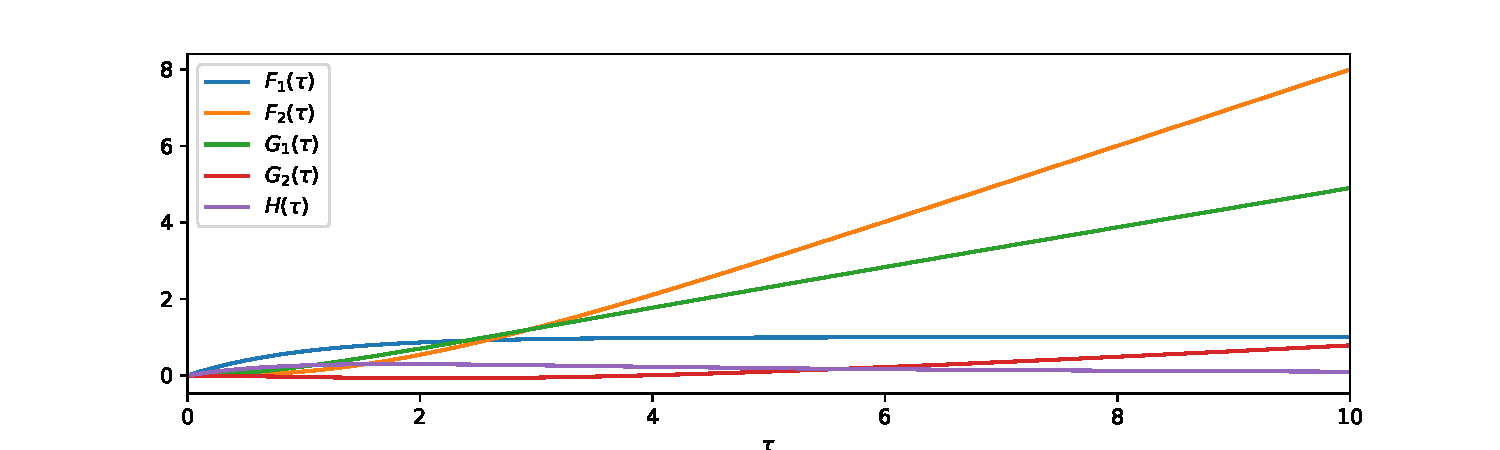
\includegraphics[width=0.90\linewidth]{exponentials/exponential-functions}
        \caption{The exponential functions, \cref{eqs:LSMOC:ET:Exponential Functions}, from 0 to 10.\label{fig:Exponential Functions}}
    \end{figure}

    These functions all involve an exponential, $e^{-\segopt}$; although this does not present a problem mathematically, the exponential function is a transcendental function that tends to be slow when evaluated computationally.
    For efficient transport codes, this presents a challenge.
    Previous works have demonstrated that function interpolation can provide significant run-time reduction \cite{Yamamoto2004}, and the original formulation \cite{Ferrer2016} suggested the use of function interpolation (though no details were provided).

    \subsection{First Approach: Improved Accuracy}{\label{ssec:LSMOC:ET:First Approach: Improved Accuracy}
      With the implementation of \ac{LSA} into MPACT, stability issues were observed in problems with very small transport cross sections, such as the fuel-clad gap in \acp{LWR}.
      These stability issues were only observed when exponential function interpolation was used, and the simplest method for addressing the issue was to increase the accuracy of the exponential interpolation.
      It was discovered that the root of the problem was the $F_2(\segopt)$ function in the transmission equation
      \begin{equation}\label{eq:LSMOC:ET:Transmission Original}
        \afluxout = \afluxin
                  + \left(\frac{\tsrcF}{\xst}-\afluxin\right)F_1(\segopt)
                  + \frac{\tsrcL}{2\left(\xst\right)^2}F_2(\segopt).
      \end{equation}
      In MPACT, source terms are actually computed and stored as $q/\xst$; however the $F_2(\segopt)$ term has an additional inverse $\xst$.
      In problems with near-void regions, where $\xst$ is small, any error in $F_2(\segopt)$ interpolation will be magnified.
      The simplest approach is to increase the accuracy of the exponential interpolation to account for the lowest expected cross sections; in the test problem this was on the order of $10^{-5}$.
      Thus, the expectation is that an interpolation 5 orders of magnitude more accurate than previous accuracy would be sufficient.
      Previous work \cite{Yamamoto2004} indicated that for \ac{FSMOC} calculations an max interpolation error of $10^{-7}$ was sufficient, i.e. for \ac{LSMOC} the max error would be within $10^{-12}$.

      Creating interpolation tables with the necessary accuracy for these problems requires some care.
      The original investigation of exponential interpolation for transport calculations  done by \citet{Yamamoto2004} indicated two methods of controlling interpolation accuracy.
      One method to increase interpolation accuracy is to increase the number of intervals (decreased interval width); however, this increased the memory.
      Alternatively, higher order polynomials can be used in the interpolation, which overall tends to reduce memory at the expense of increased run-times.

      In this investigation, two additional methods for controlling accuracy were investigated: interpolation node choice, and non-uniform interval widths.
      \subsubsection{Interpolation Points}{\label{sssec:ET:Interpolation Points}
        Within each interval of an interpolation table, the function is computed at interpolation points and an approximation of the function is made as the polynomial passing through these points.
        The placement of these points within each interval can greatly affect the accuracy of the approximation.
        Previous works \cite{Yamamoto2004,Kochunas2013} used evenly spaced interpolation points within each interval; however, this does not minimize the error in the approximation.
        An example is shown in \cref{fig:LSMOC:ET:Interpolation Example}.

        \begin{figure}
          \centering
          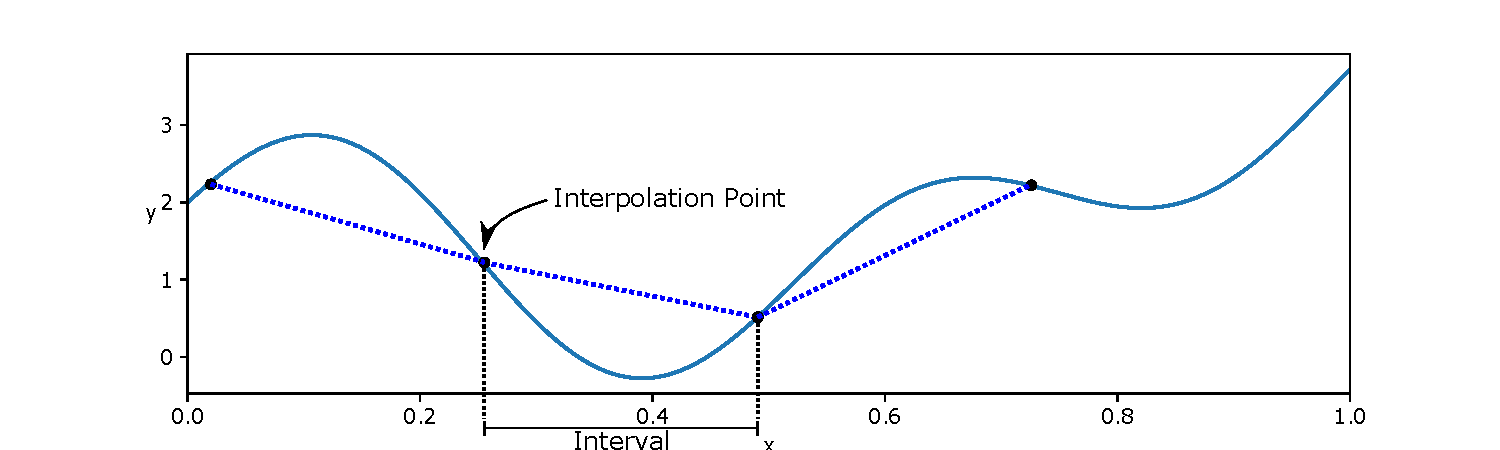
\includegraphics[width=0.90\linewidth]{exponentials/interpolation-example}
          \caption{Example of linear interpolation with uniform interval widths and interpolation points on the edge of the domain.\label{fig:LSMOC:ET:Interpolation Example}}
        \end{figure}

        Let $P_n(x)$ be the order $n$ polynomial approximating a function, $f(x)$, on an arbitrary interval $[a,b]$.
        The maximum error, $\epsilon$, within an interval is given by
        \begin{equation}\label{eq:LSMOC:ET:Interpolation Error}
          \epsilon = \frac{1}{(n+1)!}\left(\max_{\xi\in[a,b]}\lrabs{f^{(n+1)}(\xi)}\right)\left(\max_{x\in[a,b]}\lrabs{\prodl[j=1][n+1](x-x_j)}\right),
        \end{equation}
        for some value $\xi\in[a,b]$, where $f^{(n+1)}$ is the $n+1$-th derivative of $f(x)$.
        The choice of interpolation points will only affect the last term enclosed in parentheses.

        The Chebyshev points \cite{Stewart1996} are a set of values in $[a,b]$ that minimize $\max_{x\in[a,b]}\lrabs{\prodl[j=1][n+1](x-x_j)}$, and are given by
        \begin{equation}\label{eq:LSMOC:ET:Chebyshev Points}
          x_k = \frac{1}{2}\left[(a+b)+(b-1)\cos\left(\frac{2k-1}{2(n+1)}\pi\right)\right], \forall k\in\{1,2,...,n,n+1\}.
        \end{equation}
        By using the Chebyshev points, the maximum interpolation error, $\epsilon$, can be simplified to
        \begin{equation}\label{eq:LSMOC:ET:Chebyshev Interpolation Error}
          \epsilon = \frac{1}{2^n(n+1)!}\left(\frac{b-a}{2}\right)^{n+1}\max_{\xi\in[a,b]}\lrabs{f^{(n+1)}(\xi)}.
        \end{equation}
        Because the Chebyshev points do not include the end-points of the interval, there is additional cost in setting up the interpolation table, but this is negligible to typical \ac{MOC} calculation times.
        An interpolation table using Chebyshev points \emph{reduces error at no run-time cost} compared to a table using evenly spaced points.
        For this reason, Chebyshev points will be assumed for the remainder of this section.
        \Cref{tab:LSMOC:ET:Chebyshev Error} shows maximum errors for $F_1(\opt)$ interpolation for uniformly spaced points and Chebyshev points for an interval width $\Delta=b-a$.
        \begin{table}
          \centering
          \renewcommand{\arraystretch}{1.45}
          \caption{Maximum error in $F_1(\opt)$ for interval width $\Delta$.}
          \label{tab:LSMOC:ET:Chebyshev Error}
          \begin{tabular}{@{}ccc@{}}\toprule
            Polynomial Order & Uniform points   & Chebyshev points\\\midrule
            1                & $\frac{\Delta^2}{8}$           & $\frac{\Delta^2}{16}$\\
            2                & $\frac{\Delta^3}{72\sqrt{3}}$  & $\frac{\Delta^3}{192}$\\
            3                & $\frac{\Delta^4}{1536}$        & $\frac{\Delta^4}{3072}$\\\bottomrule
          \end{tabular}
        \end{table}
      }
      \subsubsection{Interval Width}{\label{sssec:LSMOC:ET:Interval Width}
        The conventional approach for interpolation tables has been to use a constant interval width, $\Delta$, for all intervals in the domain.
        This interval width is then used to control the error of the table.
        \Cref{eq:LSMOC:ET:Interpolation Error} shows that the interval bounds affect the interpolation error through the derivative term.
        The second and higher order derivatives of each of the exponential functions (\cref{eqs:LSMOC:ET:Exponential Functions}) approach zero as $\segopt$ approaches infinity.
        This indicates that the interpolation error typically decreases as the optical thickness increases in the conventional approach.

        However, is is possible to maintain the same maximum error over each interval if a variable interval width, $\Delta_i$, is used, where $i$ indicates the interval index.
        By using a variable interval width, a table can use fewer intervals while maintaining the same maximum error.
        However, since the widths are no longer constant, there is no longer a simple/direct conversion from $\segopt$ to $i$.
        Although there may be better ways, for this work the smallest interval is used to break up the domain into a map which points to the correct interval for that range of values.

        It was found that the use of non-uniform interval widths allowed for significantly fewer total intervals, reducing the memory usage, but incurring overhead for the additional mapping to index.
        \Cref{fig:LSMOC:ET:Memory Analysis} shows the memory usage for a polar-independent interpolation table for $F_1(\segopt)$.
        Using a non-uniform table typically decreases the memory usage by nearly an order of magnitude.
        For polar-dependent tables, the memory usage will be multiplied by the largest inverse sine of the polar angle, and the number of polar angles.

        \begin{figure}
          \centering
          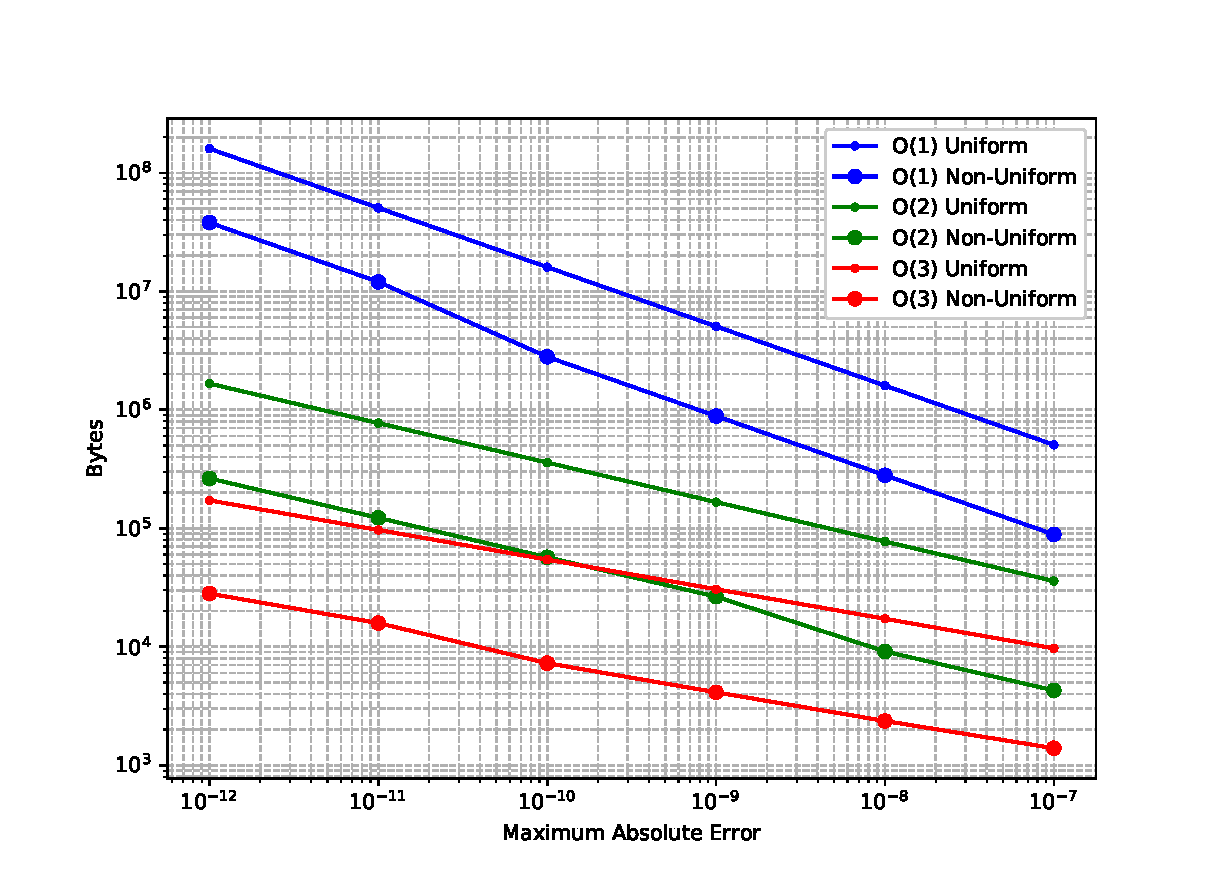
\includegraphics[width=0.90\linewidth]{exponentials/MemoryAnalysis}
          \caption{The memory usage of a single interpolation table (polar independent) for $F_1(\segopt)$ is shown as a function of the maximum error for different interpolation orders and tabulation methods.\label{fig:LSMOC:ET:Memory Analysis}}
        \end{figure}

        Because all the functions of \cref{eqs:LSMOC:ET:Exponential Functions} are related, it is possible to tabulate only a single function and compute the others from the resulting interpolated value.
        However, if $F_1(\segopt)$ is known accurately, it is not possible to compute $H(\segopt)$ for very small $\segopt$ due to round-off errors.
        Instead one can tabulate $H(\segopt)$ and use the result to compute the other functions; however, this may incur more error than directly interpolating these functions.
      }
    }
    \subsection{Function Modification}{\label{ssec:LSMOC:ET:Function Modification}
      A second approach for addressing the instability due to inaccurate function interpolation was taken: change the functions.
      Recall that the highly accurate interpolation tables of \cref{ssec:LSMOC:ET:First Approach: Improved Accuracy} were necessary due to the inverse total (or transport) cross section on the $F_2(\segopt)$ term of \cref{eq:LSMOC:ET:Transmission Original}.
      Manipulating this term, we define a new function
      \begin{equation}\label{eq:LSMOC:ET:F2 Modified Definition}
        \frac{F_2(\segopt)}{\xst} = \nlen\modFunc,
      \end{equation}
      where
      \begin{equation}\label{eq:LSMOC:ET:F2 Modified}
        \modFunc \defined 2\left(1-\frac{F_1(\segopt)}{\segopt}\right) - F_1(\segopt).
      \end{equation}
      The $\modFunc$ function can be tabulated in place of $F_2(\segopt)$; this will require an additional multiplication by the segment length $\nsegl$ causing slight reduction in performance.
      But, by using the modified $\modFunc$ function, the underlying cause of the numerical instability is addressed, and the more accurate interpolation is no longer necessary.

      One approach is to tabulate the $\modFunc$ function in place of the $F_2(\segopt)$ function, and multiply by $\nsegl$ during evaluation.
      However, as stated in the previous section, it is possible to tabulate a single function and compute the others.
      The $H(\segopt)$ function could be tabulated again; but tabulating an intermediate function,
      \begin{equation}\label{eq:LSMOC:ET:E1}
        E_1(\segopt) \defined \frac{1-e^{-\segopt}}{\segopt},
      \end{equation}
      uses the same number of operations to compute the other functions.
      This $E_1(\segopt)$ function also has smaller derivative terms around $\segopt=0$, allowing for larger interval widths with no loss in accuracy.
      Therefore, it is expected that $E_1(\segopt)$ tabulation will be more efficient.
    }
    \subsection{Results}{\label{ssec:LSMOC:ET:Results}
      The results of this section were generated in serial on a Linux system with an Intel Xeon E3-1241 v3 (3.50 GHz) processors with 8 MB L3 cache.
      Results were generated for a 2-D \ac{MOC} transport calculation.
      In 2-D it is sometimes convenient to store separate interpolation tables for each polar angle.
      Both polar dependent and independent tables were tested.

      In both of the results sections, results were generated using tables for the three functions ($F_1(\segopt)$, $F_2(\segopt)$, $H(\segopt)$), or a single function (which is then used to compute the others).
      In the results, it is considered 3 functions, as the $G_1(\segopt)$, and $G_2(\segopt)$ functions are only used in pre-computing coefficients, and not in the main \ac{MOC} solver routine.

      \subsubsection{Results using More Accurate Tables}{\label{sssec:LSMOC:ET:Results using More Accurate Tables}
        \Cref{tab:LSMOC:ET:Naive Results} shows results for the different interpolation methods in a 2-D \ac{MOC} calculation.
        The use of non-uniform intervals significantly reduced the memory usage, but the run-times generally increased.
        This is likely due to the overhead from the additional index mapping operation; it is possible that a more efficient index mapping would change these results.

        The linear tables were significantly slower than higher-order interpolations, and the non-uniform linear tables were actually slower than just using the builtin transcendental functions.
        The poor performance is due to the main memory accesses caused by the table size exceeding the largest (L3) cache size.
        The polar independent tables were faster only in the case of the linear tables, due primarily to the reduction in memory.
        In all other cases the polar-dependent tables were able to more efficiently approximate the functions.
        Using either second or third order tables gave reasonably low run-times; compared to the analytic evaluations the order 2 uniform polar dependent table led to $\sim 3.5$x speed-up in the exponential time, and $\sim 1.9$x speed-up in the overall \ac{MOC} run-time.
        The results for both second and third order interpolation tables did not vary significantly, the second order was slightly faster for uniform tables.

        However, if a single function is tabulated and used to compute the others, the memory footprint of the interpolation tables can be significantly reduced.
        Moreover, the memory accesses are reduced in favor of floating point operations which increases the computational intensity and temporal cache locality of the implementation.
        Generally, this is a favorable strategy for improving code performance as a memory access is expected to take \emph{at minimum} the same time as a single \ac{FLOP}, with cache-misses increasing that time.
        Indeed, \cref{tab:LSMOC:ET:Naive Results} shows that tabulating the single function reduced run-time in all cases.

        \begin{table}
          \centering
          \caption{Results for different exponential function evaluation methods. Maximum interpolation error of $10^{-12}$. ``w/ pol'' indicates a table with polar dependence, and ``w/o pol'' indicates a table without polar dependence.}
          \label{tab:LSMOC:ET:Naive Results}
          \footnotesize
          \begin{tabular}{@{}ccrrrrrrrrr@{}}\toprule
            Method & Table Type & Order & \multicolumn{2}{c}{\shortstack[c]{Exponential\\Time (s)}} & & \multicolumn{2}{c}{\ac{MOC} Time (s)} && \multicolumn{2}{c}{Intervals (Memory)}\\\cmidrule{4-5}\cmidrule{7-8}\cmidrule{10-11}
                  &            &       & w/ pol & w/o pol & \phantom{}                           & w/ pol & w/o pol & \phantom{}  &  \multicolumn{1}{c}{w/ pol} & \multicolumn{1}{c}{w/o pol}\\\midrule
            Analytic & N/A & N/A & \multicolumn{2}{c}{432.5} && \multicolumn{2}{c}{654.7} && \multicolumn{2}{c}{N/A}\\\midrule
            \multirow{6}{*}{3-Functions}     & \multirow{3}{*}{Uniform}        & 1 & 382.6 & 360.3 && 622.5 & 591.0 && 6.00E7 (8.04 GB) & 1.00E7 (458 MB) \\\addlinespace[-0.2em]
                                                                              && 2 & 121.3 & 151.7 && 343.2 & 372.1 && 416080 (85.7 MB) & 69360  (4.8 MB) \\\addlinespace[-0.2em]
                                                                              && 3 & 124.1 & 169.0 && 347.5 & 388.7 && 32280  (9079 KB) & 5400   (506 KB) \\\cmidrule{2-11}\addlinespace[-0.2em]
                                                & \multirow{3}{*}{Non-Uniform} & 1 & 592.9 & 559.2 && 825.8 & 800.6 && 4.07E6  (878 MB) & 840658 (76.6 MB)\\\addlinespace[-0.2em]
                                                                              && 2 & 144.6 & 178.5 && 364.3 & 397.8 && 45265  (10.9 MB) & 8020    (835 KB)\\\addlinespace[-0.2em]
                                                                              && 3 & 139.6 & 199.8 && 358.5 & 420.0 && 4491    (1.4 MB) & 796    (85.2 KB)\\\midrule
            \multirow{6}{*}{1-Function}       & \multirow{3}{*}{Uniform}       & 1 & 296.2 & 259.3 && 523.9 & 484.5 && 6.00E7 (2.68 GB) & 1.00E7  (153 MB)\\\addlinespace[-0.2em]
                                                                              && 2 &  91.4 & 123.2 && 310.2 & 345.7 && 416080 (28.6 MB) & 69360  (1.59 MB)\\\addlinespace[-0.2em]
                                                                              && 3 &  87.2 & 133.2 && 305.4 & 353.6 && 32280  (2.96 MB) & 5400    (169 KB)\\\cmidrule{2-11}\addlinespace[-0.2em]
                                                & \multirow{3}{*}{Non-Uniform} & 1 & 474.6 & 424.0 && 714.6 & 653.9 && 4.07E6  (415 MB) & 722899 (49.2 MB)\\\addlinespace[-0.2em]
                                                                              && 2 & 105.8 & 146.4 && 326.6 & 367.7 && 41444   (4.4 MB) & 7338   (443  KB)\\\addlinespace[-0.2em]
                                                                              && 3 &  98.9 & 153.3 && 318.8 & 373.2 && 4152    (515 KB) & 735    (33.5 KB)\\\bottomrule
          \end{tabular}
        \end{table}
      }
      \subsubsection{Results using Modified Function}{\label{sssec:LSMOC:ET:Results using Modified Function}
        Results were generated for the same cases as the more accurate table, but the interpolation accuracy was $10^{-7}$ rather than $10^{-12}$, as the function modification addressed the cause of the instability.
        The results are summarized in \cref{tab:LSMOC:ET:Final Results}.
        In one approach the three functions are tabulated, in the other $E_1(\segopt)$ is tabulated and used to compute the three functions.
        Previous results showed that the polar-independent and non-uniform interval width tables were slower than uniform polar-dependent tables; here the results are only shown for the uniform polar-dependent interpolation tables.

        The interpolation accuracy is not required to be as high as in the previous cases, thus the tables are significantly smaller in memory size.
        The linear tables no longer exceed the L3 cache size and are not prohibitively slow to use.
        In fact, the linear tables are the fastest option for both 3-table and single-table interpolation methods.
        Interpolating $E_1(\segopt)$ and computing the other functions from the result was the fastest approach overall.
        As before, this is expected because this method favors \acp{FLOP} over memory accesses.

        This approach also significantly reduces the number of intervals necessary (by about 3 orders of magnitude).
        Although the higher-order interpolation ended up not being more efficient than the linear interpolation tables, the number of intervals is extremely small.
        These methods may be useful on different architectures (such as \acp{GPGPU}\footnote{this statement was not confirmed as part of this study, and is speculation based on knowledge of architecture constraints.}) where memory is more limited than on a single-threaded \ac{CPU} calculation.

        \begin{table}
          \centering
          \caption{Results using the modified $\modFunc$ function, with maximum interpolation error of $10^{-7}$. Memory is under 1 MB in all cases.}
          \label{tab:LSMOC:ET:Final Results}
          \begin{tabular}{@{}ccccc@{}}\toprule
            Method & Order & Exp.     & \ac{MOC}& \# Intervals \\
                   &       & Time (s) & Time (s) & \\\midrule
            \multirow{3}{*}{3-Functions}      & 1 &  88.4 & 307.9 & 4774\\
                                              & 2 &  99.7 & 316.8 &  225\\
                                              & 3 & 116.5 & 333.1 &   46\\\midrule
            \multirow{3}{*}{$E_1(\opt)$ Only} & 1 &  80.5 & 299.0 & 2739\\
                                              & 2 &  87.6 & 307.3 &  158\\
                                              & 3 &  99.0 & 317.7 &   38\\\bottomrule
          \end{tabular}
        \end{table}
      }
    }
    %%%%%%%%%%%%%%%%%%%%%%%%%%%%%%%%%%%%%%%%%%%%%%%%%%%%%%%%%%%%%%%%%%%%%%%%%%%%
    % Conclusions
    %%%%%%%%%%%%%%%%%%%%%%%%%%%%%%%%%%%%%%%%%%%%%%%%%%%%%%%%%%%%%%%%%%%%%%%%%%%%
    \subsection{Conclusions}{\label{ssec:LSMOC:ET:Conclusions}
      This study focused on the investigation of efficient approximation of the exponential functions in the \ac{LSMOC}.
      Methods for efficiently approximating the exponential function for \ac{FSMOC} have previously been investigated.
      However, these methods, applied without modification to the \ac{LSMOC} can lead to numerical instability in problems with near-void regions.
      One approach to deal with these instabilities is to improve the accuracy of the interpolation tables based on the lowest cross section in the problem.
      While this approach can be made efficient, if cross sections become too small the tables may become exceedingly large and significantly hamper performance.

      This investigation revealed that the cause of the instability was the $F_2(\segopt)$ function in the transmission equation.
      By instead manipulating the term including this function, the cause of the instabilities can be addressed.
      This approach no longer requires excessively large interpolation tables; however, some key-findings from the first approach can be applied to make this appraoch faster.
      First, the use of Chebyshev points significantly increases interpolation accuracy for the same number of intervals as uniformly spaced points, at no run-time cost.
      Additionally, by interpolating a single function and using the result to compute the other functions performance can be significantly improved.
    }
  }
  %%%%%%%%%%%%%%%%%%%%%%%%%%%%%%%%%%%%%%%%%%%%%%%%%%%%%%%%%%%%%%%%%%%%%%%%%%%%%%
  % Improved Linear Source Formulation for Multi-physics and 2D/1D Applications
  %%%%%%%%%%%%%%%%%%%%%%%%%%%%%%%%%%%%%%%%%%%%%%%%%%%%%%%%%%%%%%%%%%%%%%%%%%%%%%
  \section{Improved Linear Source Formulation for Multi-physics and 2D/1D Applications}{\label{sec:Improved Linear Source Formulation for Multi-physics and 2D/1D Applications}
    As stated in \cref{sec:MOC:LSA}, the original derivation of the moment-based \acf{LSA} from \citet{Ferrer2016} faced inefficiencies in problems with non-constant cross sections.
    The inefficiencies arose from the use of pre-computed coefficients, \cref{eq:MOC:LSA:C Matrix}, which must be re-computed if cross sections change.
    In multiphysics calculations, such as with \ac{TH} feedback, cross sections typically change each iteration, leading to significant overhead from re-computing these terms.
    This section presents and equivalent formulation, which eliminates the need to re-compute these terms if cross sections change, without additional operations.

    \subsection{Derivation}{\label{ssec:LSMOC:Derivation}
      The derivation of this improved formulation begins with the same initial steps as the derivation detailed in \cref{ssec:MOC:LSA:Derivation}.
      Several of these equations are repeated in this section for clarity.
      The source is assumed to have a spatially linear shape
      \begin{equation}\label{eq:LSMOC:Source Shape}
        \source[mi][g][\loc] \approx \srcF[mi] + \loc\vdot\srcL[][mi],
      \end{equation}
      and the angular flux moments can be expanded similarly
      \begin{equation}\label{eq:LSMOC:Flux Expansion}
        \fluxA(\loc) = \fluxF + \loc\vdot\fluxL.
      \end{equation}
      The source can be computed from the flux moments using \cref{eq:MOC:LSA:Linear Source Computation}.

      Computing the source requires the flux to be evaluated during transport sweeping.
      The angular flux moments are given by \cref{eqs:MOC:LSA:Region-Averaged Flux Moments Definitions}, but are repeated here for clarity.
      \begin{subequations}\label[subeqs]{eqs:LSMOC:Region-Averaged Flux Moments Definitions}
        The spatially flat angular flux moments are defined by integrating the flux multiplied by a spherical harmonics moment function over space and directions,
        \begin{equation}\label{eq:LSMOC:Region-Averaged Flux Moment Definition}
            \fluxF \defined \MOCIntegral{\SH \aflux[][g][]} = \frac{\fourpi}{V_i}\suml[m]\wt\SH[\ell][n][\dirm]\suml[k]\tA[mki]\nsegl\MOCTrackIntegral{\aflux[][g][]}.
        \end{equation}
        To determine the spatial expansion coefficients of the flux moments, \cref{eq:LSMOC:Flux Expansion} is operated on by $\MOCIntegral{\SH\loc(\vdot)}$.
        As before, this should be directly proportional to the angular flux operated on by $\MOCIntegral{\SH\loc\aflux[][g][]}$, a system of equations is found
        \begin{equation}\label{eq:LSMOC:Moment to Expansion Coefficient}
            \M\fluxL = \MOCIntegral{\SH\loc\aflux[][g][]},
        \end{equation}
        where
        \begin{equation}\label{eq:LSMOC:Geometric Moments}
            \M \defined \MOCIntegral{\loc^T\loc}.
        \end{equation}
        The spatial angular flux moments, $\MOCIntegral{\SH\loc\aflux[][g][]}$, are then defined as
        \begin{equation}\label{eq:LSMOC:Region-Averaged Spatial Angular Flux Moments Definition}
            \MOCIntegral{\SH\loc\aflux[][g][]} = \frac{\fourpi}{V_i}\suml[m]\wt\SH[\ell][n][\dirm]\suml[k]\tA[mki]\nsegl\left(\locIn\MOCTrackIntegral{\aflux[][g][]} + \dirm\MOCTrackIntegral{\nlen\aflux[][g][]} / \renorm[mi]\right).
        \end{equation}
      \end{subequations}

      With the assumed source shape, \cref{eq:LSMOC:Source Shape}, the characteristic transport equation becomes
      \begin{subequations}\label[subeqs]{eqs:LSMOC:Characteristic Form}
        The characteristic transport equation becomes
        \begin{equation}\label{eq:LSMOC:Characteristic Form}
          \left[\deriv{}{\nlen} + \xst\right]\aflux = \tsrcF + \tsrcL\left(\nlen - \frac{\nsegl}{2}\right),
        \end{equation}
        where
        \begin{equation}\label{eq:LSMOC:Track Average Source}
          \tsrcF \defined \rfourpi\left[\srcF[mi] + \locCent \vdot \srcL[][mi]\right],
        \end{equation}
        \begin{equation}\label{eq:LSMOC:Track Linear Source}
          \tsrcL \defined \rfourpi\left[\frac{\dirm\vdot\srcL[][mi]}{\renorm[mi]}\right],
        \end{equation}
        and $\locCent$ is the local-coordinate centroid of the track-segment.
      \end{subequations}
      Substituting this assumed source shape (linear) into the generic \ac{MOC} solution, given by \cref{eq:MOC:MOC Generic Solution}, the angular flux along a track-segment is found to be
      \begin{subequations}\label[subeqs]{eqs:LSMOC:Angular Flux Solution}
          \begin{equation}\label{eq:LSMOC:Angular Flux Solution}
              \aflux = \afluxin + \left(\frac{\tsrcF}{\xst} - \afluxin\right)F_1(\opt) + \frac{\tsrcL}{2(\xst)^2}F_2(\opt),
          \end{equation}
          where
          \begin{equation}\label{eq:LSMOC:F1}
              F_1(\opt) \defined 1 - \exp(-\opt),
          \end{equation}
          and
          \begin{equation}\label{eq:LSMOC:F2}
              F_2(\opt) \defined 2[\opt-F_1(\opt)] - \segopt F_1(\opt).
          \end{equation}
      \end{subequations}

      To evaluate the moments defined in \cref{eqs:LSMOC:Region-Averaged Flux Moments Definitions}, the track-average flux and first spatial moment of the angular flux must be determined.
      \begin{subequations}\label[subeqs]{eqs:LSMOC:Flux Track Moments}
        The track-average flux is determined as it was before, by operating on \cref{eq:LSMOC:Characteristic Form} by $\nsegl\MOCTrackIntegral{(\vdot)}$, yielding
        \begin{equation}\label{eq:LSMOC:0th Track Moment of the Flux}
          \MOCTrackIntegral{\aflux[][g][]} = \frac{\tsrcF}{\xst} + \frac{\dflux}{\segopt}.
        \end{equation}
        At this point the two derivations diverge from one another.
        In the previous formulation, the integral in $\MOCTrackIntegral{\nlen\aflux[][g][]}$ is \emph{explicitly} evaluated by substituting in the solution of the angular flux along the track (\cref{eqs:MOC:LSA:Angular Flux Solution}).
        Here, the moment will be found implicitly by operating on \cref{eq:LSMOC:Characteristic Form} by $\nsegl\MOCTrackIntegral{\nlen(\vdot)}$, just as was done for the 0th moment.
        This results in
        \begin{equation}\label{eq:LSMOC:1st Track Moment of the Flux}
          \MOCTrackIntegral{\nlen\aflux[][g][]} =
            \frac{\MOCTrackIntegral{\aflux[][g][]} - \afluxout}{\xst}
              + \frac{\nsegl}{2}\left[\frac{\tsrcF}{\xst}
              + \frac{\tsrcL}{\xst}\frac{\nsegl}{6}\right].
        \end{equation}
        Unlike \cref{eq:MOC:LSA:Track-Averaged Linear Angular Flux}, there a not any new exponential functions introduced in this form.
      \end{subequations}

      Previously, the average track flux, $\MOCTrackIntegral{\aflux[][g][]}$, was expanded to find a simpler final form.
      This is the case here as well; however, the out-going flux, $\afluxout$, will not be expanded, as this must necessarily be computed during transmission.
      \Cref{eqs:LSMOC:Region-Averaged Flux Moments Definitions} can be simplified into
      \begin{subequations}\label[subeqs]{eqs:LSMOC:Region-Averaged Flux Moments}
        \begin{equation}\label{eq:LSMOC:Region-Averaged Flat Flux Moments}
          \fluxF = \frac{\fourpi}{V_i\xst}\suml[m]\wt\SH\suml[k]\tA\left(\nsegl\tsrcF + \dflux\right),
        \end{equation}
        and
        \begin{aequation}\label{eq:LSMOC:Region-Averaged Linear Flux Moments}
          \MOCIntegral{\SH\loc\aflux[][g][]}
            = &\frac{1}{V_i}\suml[m]\wt\SH\suml[k]\tA\nsegl\left[\locCent\srcF + \left(\locCent(\locCent)^T + \frac{\segl^2}{12}\dirm\dirm^T\right)\srcL\right]\\
            + &\frac{\fourpi}{V_i\xst}\suml[m]\wt\SH\suml[k]\tA\left[\locIn\dflux + \dirm\segl\left(\frac{\dflux}{\segopt}-\afluxout+\frac{\tsrcF}{\xst}\right)\right]
        \end{aequation}
      \end{subequations}

      \Cref{eq:LSMOC:Region-Averaged Linear Flux Moments} contains $\dflux/\segopt$ terms, rather than only $\dflux$ terms.
      For numerical stability, it is beneficial to compute this quantity directly, rather than $\dflux$ and performing division.
      This can be found by evaluating the transmission equation, \cref{eq:LSMOC:Angular Flux Solution}, giving
      \begin{subequations}\label[subeqs]{eqs:LSMOC:Average Slope}
        \begin{equation}\label{eq:LSMOC:Average Slope}
          \frac{\dflux}{\segopt} = \left(\afluxin-\frac{\tsrcF}{\xst}\right)E_1(\segopt) - \frac{\nsegl}{2}\frac{\tsrcL}{\xst}T_2(\segopt),
            \end{equation}
            where
            \begin{equation}\label{eq:LSMOC:E1}
                E_1(\segopt) \defined \frac{F_1(\segopt)}{\segopt},
            \end{equation}
            \begin{equation}\label{eq:LSMOC:T2}
                T_2(\segopt) \defined 2E_2(\segopt) - E_1(\segopt),
            \end{equation}
            and
            \begin{equation}\label{eq:LSMOC:E2}
                E_2(\segopt) \defined \frac{1-E_1(\segopt)}{\segopt}.
            \end{equation}
      \end{subequations}
      Here, $E_2(\segopt)$ is defined as an intermediate function which has smaller derivative terms, meaning higher accuracy with fewer interpolation intervals (see \cref{sec:LSMOC:Exponential Tabulation}).
      Following the conclusions of \cref{sec:LSMOC:Exponential Tabulation}, only the $E_2(\segopt)$ function needs to be tabulated, and then is used to compute the other two exponential functions, $E_1(\segopt)$, and $T_2(\segopt)$.
      The outgoing flux can then be evaluated as
      \begin{equation}\label{eq:LSMOC:Outgoing Flux}
        \afluxout = \afluxin - \segopt\frac{\dflux}{\segopt}.
      \end{equation}
    }
    \subsection{Particle Conservation}{\label{ssec:LSMOC:Particle Conservation}
      As described in \cref{ssec:MOC:LSA:Particle Conservation}, particle conservation puts the constraint of using direction-dependent renormalization and centroids, in addition to directional quadrature constraints.
      If these constraints are satisfied, \cref{eqs:LSMOC:Region-Averaged Flux Moments} can be simplified into
      \begin{subequations}\label[subeqs]{eqs:LSMOC:Conservation:Region-Averaged Flux Moments}
        \begin{equation}\label{eq:LSMOC:Conservation:Region-Averaged Flat Flux Moments}
          \fluxF = \suml[m]\wt\SH\frac{\srcF}{\xst} + \frac{\fourpi}{V_i\xst}\suml[m]\wt\SH\suml[k]\tA\dflux,
        \end{equation}
        and
        \begin{aequation}\label{eq:LSMOC:Conservation:Region-Averaged Linear Flux Moments}
          \MOCIntegral{\SH\loc\aflux[][g][]} =
            &\suml[m]\wt\SH\M[][mi]\frac{\srcL}{\xst}\\
            +& \frac{\fourpi}{V_i\xst}\suml[m]\wt\SH\suml[k]\tA\left[\locIn\dflux + \dirm\segl\left(\frac{\dflux}{\segopt}-\afluxout+\frac{\tsrcF}{\xst}\right)\right],
        \end{aequation}
        where
        \begin{equation}\label{eq:LSMOC:Direction-Dependent M}
          \M[][mi] \defined \frac{1}{V_i}\suml[k]\tA\left[\locCent(\locCent)^T+\frac{\segl^2}{12}\dirm\dirm^T\right].
        \end{equation}
      \end{subequations}

      Although the above form seems to more computationally efficient, it would be negligent for this chapter to not include a more mathematically elegant form of \cref{eq:LSMOC:Region-Averaged Linear Flux Moments}.
      The terms in the second summation may be rewritten as
      \begin{subequations}\label[subeqs]{eqs:LSMOC:Region-Averaged Linear Flux Moments Elegant}
        \begin{aequation}\label{eq:LSMOC:Region-Averaged Linear Flux Moments Elegant}
          \MOCIntegral{\SH\loc\aflux[][g][]} =&
            \suml[m]\wt\SH\M[][mi]\frac{\srcL}{\xst} \\
            &+ \frac{\fourpi}{V_i}\suml[m]\wt\SH\suml[k]\tA\left[\locIn\left(\afluxin-\tfluxF\right)-\locOut\left(\afluxout-\tfluxF\right)\right],
        \end{aequation}
        where $\tfluxF$ is the average track flux,
        \begin{equation}\label{eq:Average Track Flux}
          \tfluxF \defined \nsegl\MOCTrackIntegral{\aflux[][g][]}.
        \end{equation}
      \end{subequations}
      In this form, the interior summation over track-segments becomes a spatially weighted summation of the incident and outlet flux differences from the average flux.
    }
    \subsection{Isotropic Simplifications}{\label{ssec:LSMOC:Isotropic Simplifications}
      If the so called \acf{LIFA} scheme is used, the spatially flat moment equations do not change; however, \cref{eq:LSMOC:Region-Averaged Linear Flux Moments} can be simplified to
      \begin{aequation}\label{eq:LSMOC:LIFA:Region-Averaged Linear Flux Moments}
        \MOCIntegral{\SH\loc\aflux[][g][]} &= \M\frac{\srcL}{\xst}\\ &+ \frac{\fourpi}{V_i\xst}\suml[m]\wt\suml[k]\tA\left[\locIn\dflux+\dirm\segl\left(\frac{\dflux}{\segopt}-\afluxout+\frac{\tsrcF}{\xst}\right)\right]
      \end{aequation}
    }
  }

  \section{Results}{\label{sec:LSMOC:Results}
    \subsection{C5G7 Benchmark}{\label{ssec:LSMOC:C5G7 Benchmark}
      The 2-D C5G7 benchmark \cite{Smith2006} is a neutronics benchmark used by various codes to help verify the correctness of the solvers used.
      A 7-group cross section library of macroscopic cross sections is provided by the benchmark.
      The benchmark consists of two \ac{UO2} assemblies and two \ac{MOX} assemblies surrounded by a large radial reflector, as shown in \cref{fig:LSMOC:C5G7:CoreGeom}.
      Reflective boundary conditions are used on the north and west faces, while vacuum conditions are used on the south and east faces.
      The benchmark provides reference MCNP calculation results, which can be used to determine the accuracy of the methods used to solve the benchmark cases.

      \begin{figure}[htbp]
        \centering
        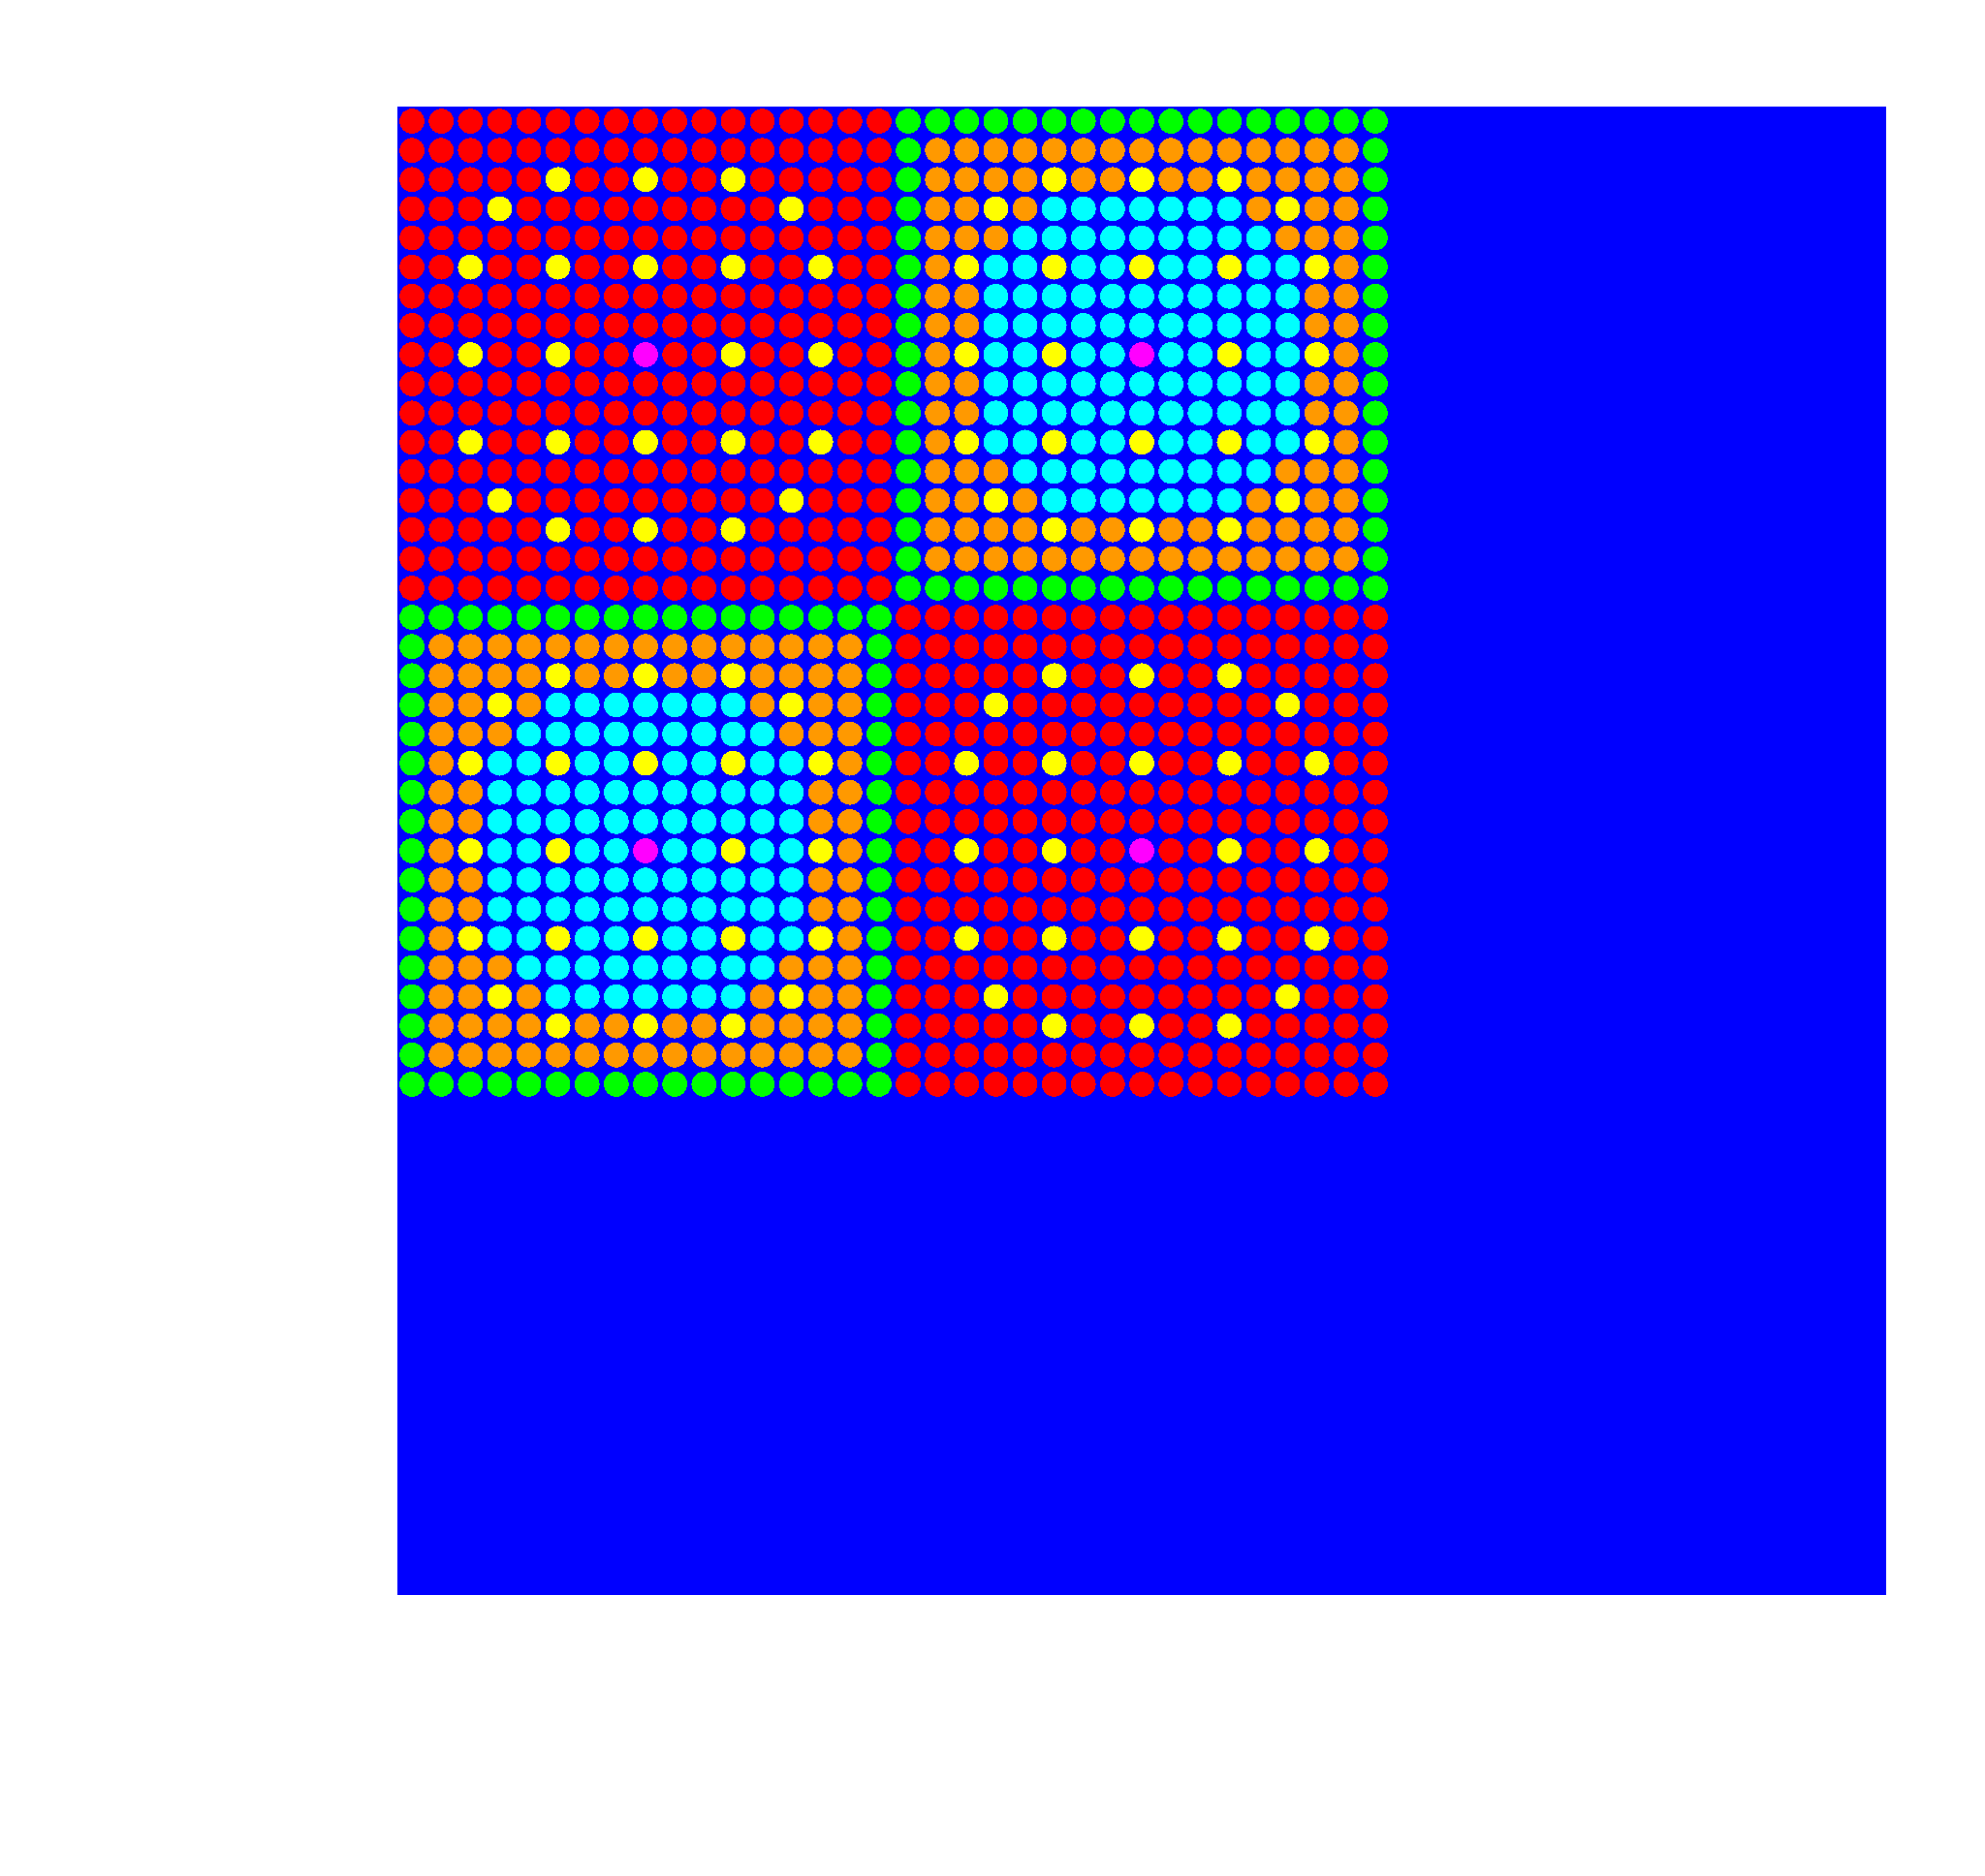
\includegraphics[width=0.45\linewidth]{\figpath/c5g7/core}
        \caption{Geometry and materials of the 2-D C5G7 benchmark. \label{fig:LSMOC:C5G7:CoreGeom}}
      \end{figure}

      This problem was studied in order to verify that the implementation of the \ac{LSA} derived in this chapter yields similar results to those found by \citet{Ferrer2016}.
      Similar meshing, ray, and direction parameters were used in this study as were used in the original study \cite{Ferrer2016}; some parameters could not be replicated exactly due to differences in the MPACT and CASMO5 codes.
      All cases used a uniform ray-spacing of 0.05 cm, and directional quadrature using 128 azimuthal angles and 6 polar angles in $\fourpi$.
      Each case was run using od\ac{CMFD} \cite{Zhu2016}.

      The fine pin cell mesh used 5 rings in the fuel region, 10 in the moderator region, and 16 azimuthal divisions in all regions.
      The fine reflector cell mesh was divided into 0.105$\times$0.105 cm$^2$ cells.
      The coarse pin cell mesh used a single fuel ring with four azimuthal divisions, and no moderator rings, using 8 azimuthal divisions in the surrounding moderator.
      The coarse reflector cell mesh was divided into 0.42$\times$0.42 cm$^2$ cells.

      Three cases were run in this study: fine mesh with \ac{FSA}, coarse mesh with \ac{FSA}, and coarse mesh with \ac{LSA}.
      To be consistent with \citet{Ferrer2016} results, it is expected that the \ac{LSA} on the coarse mesh should reduce run-time while maintaining accuracy compared to the finely mesh \ac{FSA} calculation.
      Additionally, the coarse mesh \ac{FSA} calculation should have significantly worse accuracy, thus justifying the use of the \ac{LSA}.

      \Cref{tab:LSMOC:C5G7:Results} shows very clearly that the \ac{LSA} on the coarse mesh is more accurate than the \ac{FSA} on the fine mesh.
      While \ac{FSA} on the fine mesh provides reasonable accuracy, the \ac{FSA} on the coarse mesh shows significant errors compared to the MCNP reference.
      In terms of accuracy, the results agree very closely with those reported for the original derivation of the moment-based \ac{LSA}.
      The reference pin-powers are visualized in \cref{figs:LSMOC:C5G7:Reference:PinPowers}, and the differences are shown in \cref{figs:LSMOC:C5G7:FineFS:PinPowers,figs:LSMOC:C5G7:CoarseFS:PinPowers,cpfigs:LSMOC:C5G7:CoarseLS:PinPowers}.
      The largest pin-power differences for the fine mesh with \ac{FS} and coarse mesh with \ac{LS} are in the center assembly where pin-powers are higher.
      Interestingly, the largest pin-power differences for the coares mesh with \ac{FS} case are in the pins bordering the radial reflector region;
        this indicates that the mesh in the reflector was not sufficient.
      Errors in the interior of the assemblies are still larger for this case than the others.

      \Cref{tab:LSMOC:C5G7:Performance} indicates that the \ac{LSA} on the coarse mesh significantly out performs the \ac{FSA} on the fine mesh;
      \ac{MOC} run-time is reduced by approximately 50\%, and memory usage is reduced by 45\%.
      However, this also shows that for this problem the \ac{LSA} solver takes just under 2 times the time of the \ac{FSA} on the same mesh (coarse).
      It is also shown, that there is very little memory overhead from using the \ac{LSA} on the same mesh as the \ac{FSA}.
      The number of iterations is quite different of that reported by \citet{Ferrer2016}; however, the iteration scheme in CASMO5 is different than that of MPACT \cite{FerrerPersoanlCommunications2018}.
      In MPACT, each iteration loops over all energy groups a single time, but in CASMO5 the thermal energy groups are iterated over multiple times.

      \begin{table}[htbp]
        \centering
        \caption{
          Accuracy comparisons for the C5G7 2-D benchmark calculation using different source approximations and meshes.
          In addition to eigenvalue difference, several metrics for comparing pin-powers are provided.
          The abbreviations are as follows:
            MPP+ = difference in maximum pin-power, MPP- = difference in minimum pin-power,
            AVE = average pin-power error, RMS = root-mean-square pin-power error,
            MRE = mean relative error.
          The number of pins with power within 68\% and 95\% of the MCNP reference results are also listed.
        }
        \label{tab:LSMOC:C5G7:Results}
        \begin{tabular}{rrrrrrrrrrr}\toprule
                 &      &                     & \multicolumn{6}{c}{Pin Powers (\%)} & \multicolumn{2}{c}{\# Pins within}\\
          Solver & Mesh & $\Delta\keff$ (pcm) & MPP+ & MPP- & MPE & AVE & RMS & MRE & 68\% & 95\%\\\midrule
          FSA    & Fine    & 8                & -0.13 & 0.89 & 0.98 & 0.18 & 0.24 & 0.15 & 494 & 763\\
          FSA    & Coarse  & 65               & -0.76 & 3.74 & 4.23 & 0.78 & 1.16 & 0.61 & 142 & 217\\
          LSA    & Coarse  & 2                &  0.02 & 0.30 & 0.66 & 0.12 & 0.16 & 0.10 & 663 & 901\\\bottomrule
        \end{tabular}
      \end{table}

      \begin{table}[htbp]
        \centering
        \caption{Performance comparisons for the C5G7 2-D benchmark calculation using different source approximations and meshes.}
        \label{tab:LSMOC:C5G7:Performance}
        \begin{tabular}{rrrrrr}\toprule
                 &      &            & \multicolumn{2}{c}{Run-time (s)} & \\\cline{4-5}
          Solver & Mesh & Iterations & MoC & MoC / iter  & Memory (MB)\\\midrule
          FSA    & Fine   & 13         & 435 & 33 & 409\\
          FSA    & Coarse & 11         &  89 &  8 & 213\\
          LSA    & Coarse & 13         & 209 & 16 & 223\\\bottomrule
        \end{tabular}
      \end{table}

      \begin{figure}[htbp]
        \centering
        \begin{subfigure}[t]{0.49\textwidth}
          \centering
          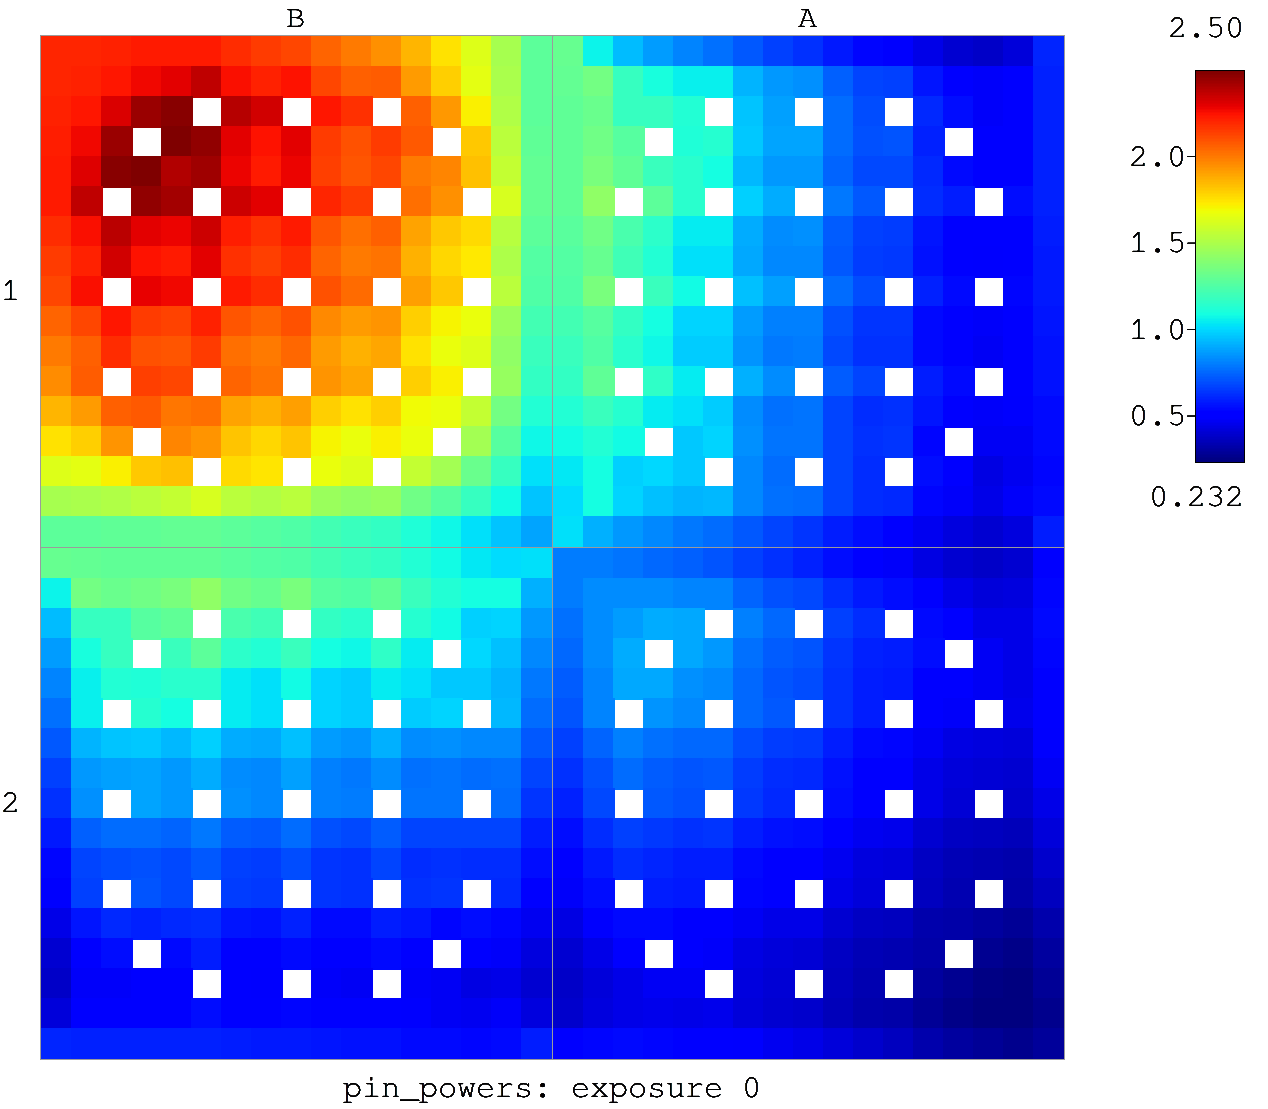
\includegraphics[width=\textwidth]{\figpath/c5g7/PinPowersCore}
          \caption{core \label{fig:LSMOC:C5G7:Reference:PinPowers:Core}}
        \end{subfigure}%
        ~
        \begin{subfigure}[t]{0.49\textwidth}
          \centering
            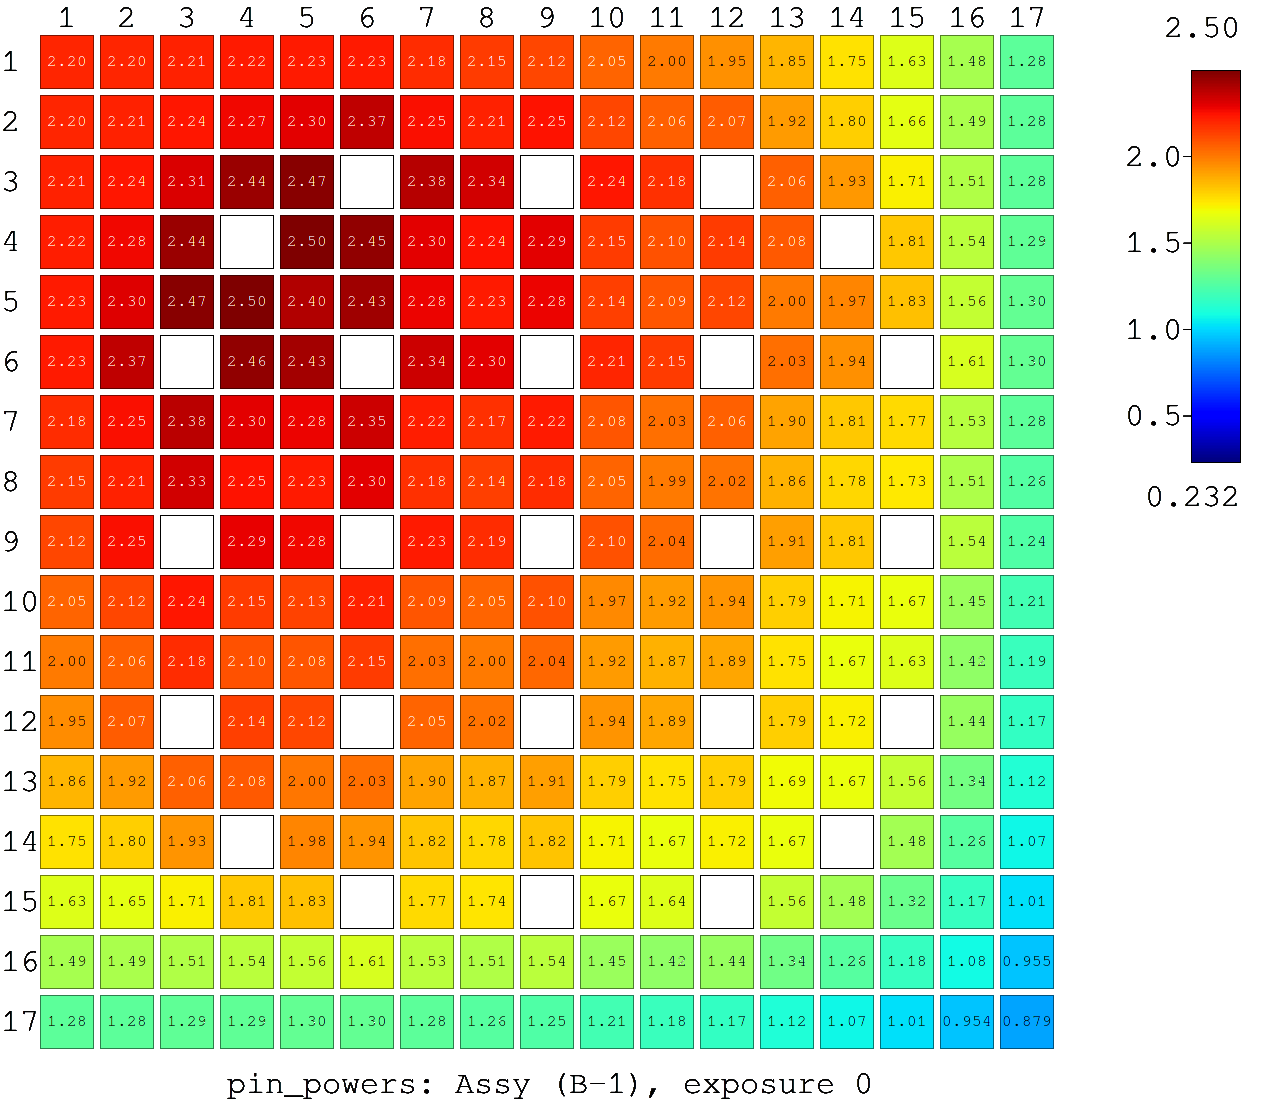
\includegraphics[width=\textwidth]{\figpath/c5g7/PinPowersAssembly}
            \caption{center assembly\label{fig:LSMOC:C5G7:Reference:PinPowers:Assembly}}
        \end{subfigure}
        \caption{Reference pin powers shown for the core and center assembly.\label{figs:LSMOC:C5G7:Reference:PinPowers}}
      \end{figure}
      \begin{figure}[htbp]
        \centering
        \begin{subfigure}[t]{0.49\textwidth}
          \centering
          \includegraphics[width=\textwidth]{\figpath/c5g7/fineFS/DiffPinPowersCore}
          \caption{core\label{fig:LSMOC:C5G7:FineFS:PinPowers:Core}}
        \end{subfigure}%
        ~
        \begin{subfigure}[t]{0.49\textwidth}
          \centering
            \includegraphics[width=\textwidth]{\figpath/c5g7/fineFS/DiffPinPowersAssembly}
            \caption{center assembly\label{fig:LSMOC:C5G7:FineFS:PinPowers:Assembly}}
        \end{subfigure}
        \caption{Pin power differences from reference shown for the core and center assembly for the fine mesh using the FSA solver.\label{figs:LSMOC:C5G7:FineFS:PinPowers}}
      \end{figure}
      \begin{figure}[htbp]
        \centering
        \begin{subfigure}[t]{0.49\textwidth}
          \centering
          \includegraphics[width=\textwidth]{\figpath/c5g7/coarseFS/DiffPinPowersCore}
          \caption{core\label{fig:LSMOC:C5G7:CoarseFS:PinPowers:Core}}
        \end{subfigure}%
        ~
        \begin{subfigure}[t]{0.49\textwidth}
          \centering
            \includegraphics[width=\textwidth]{\figpath/c5g7/coarseFS/DiffPinPowersAssembly}
            \caption{center assembly\label{fig:LSMOC:C5G7:CoarseFS:PinPowers:Assembly}}
        \end{subfigure}
        \caption{Pin power differences from reference shown for the core and center assembly for the coarse mesh using the FSA solver.\label{figs:LSMOC:C5G7:CoarseFS:PinPowers}}
      \end{figure}
      \begin{figure}[htbp]
        \centering
        \begin{subfigure}[t]{0.49\textwidth}
          \centering
          \includegraphics[width=\textwidth]{\figpath/c5g7/coarseLS/DiffPinPowersCore}
          \caption{core\label{fig:LSMOC:C5G7:CoarseLS:PinPowers:Core}}
        \end{subfigure}%
        ~
        \begin{subfigure}[t]{0.49\textwidth}
          \centering
            \includegraphics[width=\textwidth]{\figpath/c5g7/coarseLS/DiffPinPowersAssembly}
            \caption{center assembly\label{fig:LSMOC:C5G7:CoarseLS:PinPowers:Assembly}}
        \end{subfigure}
        \caption{Pin power differences from reference shown for the core and center assembly for the coarse mesh using the LSA solver.\label{figs:LSMOC:C5G7:CoarseLS:PinPowers}}
      \end{figure}
    }

    \subsection{Typical Pin Cell Depletion}{\label{ssec:LSMOC:Typical Pin Cell Depletion}
      In order to evaluate the benefits of this new formulation, the first multiphysics case studied was a typical \ac{UO2} fuel cell, as specified by \ac{VERA} progression problem 1A \cite{VERAProblems}.
      Isotopic depletion calculations were run up to 70 \ac{GWDMT} ($\sim$1820 \ac{EFPD}) at \ac{HFP} conditions.
      Using the current default meshing parameters in MPACT as a starting point, various mesh parameters were coarsened to study their affect when using the \ac{LSMOC}.
      These cases were compared against a reference case which was very finely meshed with fine ray-spacing (0.001 cm), and a Tabuchi-Yamamoto \cite{Yamamoto2005} quadrature using 128 azimuthal angles and 4 polar angles over $\fourpi$
      All other cases were run using a Tabuchi-Yamamoto quadrature with 64 azimuthal angles and 4 polar angles, with a uniform ray-spacing of 0.05 cm.

      \paragraph{Default Mesh}{
        MPACT's current default meshing parameters were used as a starting point.
        Flat and linear source calculations were run on this mesh, to set a baseline for ``acceptable'' levels of error in the eigenvalue.
        Compared to the reference case, the \ac{LS} calculation had a larger maximum error in eigenvalue of 89.2 \ac{pcm}, whereas the \ac{FS} calculation had a maximum error of 65.5 \ac{pcm}.
        However, the average errors over the depletion were approximately the same: 31.6 and 33.7 \ac{pcm}, for the \ac{FS} and \ac{LS} calculations, respectively.
        The eigenvalue differences over the depletion calculation are shown in \cref{fig:LSMOC:1a:DefaultMesh:Eigenvalue}.
        The goal in this mesh refinement study is to determine acceptable meshing parameters without worse maximum or average eigenvalue errors.

        \begin{figure}
            \centering
            \includegraphics[width=\linewidth]{1a/DefaultMesh-Eigenvalues}
            \caption{Reference eigenvalues and differences for the default mesh pin cell case with isotopic depletion. \label{fig:LSMOC:1a:DefaultMesh:Eigenvalue}}
        \end{figure}
      }
      \paragraph{Fuel Radius}{
        During isotopic depletion, it is important to accurately capture the radial distribution of Plutonium, due to self-shielding effects.
        Plutonium is primarily produced in the outer rim of the pin, this is well known as the rim-effect.
        The default mesh uses three equal volume rings in the fuel region; however, we expect that two rings will be sufficient, when using the \ac{LSA}, if the extra ring is placed in such a way that it captures this rim-effect.
        Experimental studies of the rim-effect \cite{Lassmann1994} have found that there is a sharp rise in Plutonium at around between 80-90\% of the outer radius of the fuel.

        A series of calculations were run using two fuel rings with varying inner radius.
        The eigenvalue and Plutonium comparisons are shown in \cref{fig:LSMOC:1a:FuelRadius:Eigenvalue,fig:LSMOC:1a:FuelRadius:Pu239}.
        Comparing eigenvalues, a fractional radius between 0.825 and 0.875 seem to have little effect on the mean or worst-case eigenvalue difference.
        By comparing the concentration of Pu-239, these radii are again shown to be the most accurate; a fractional radius of 0.875 was chosen to be sufficient, and used in the remainder of the studies.

        \begin{figure}
            \centering
            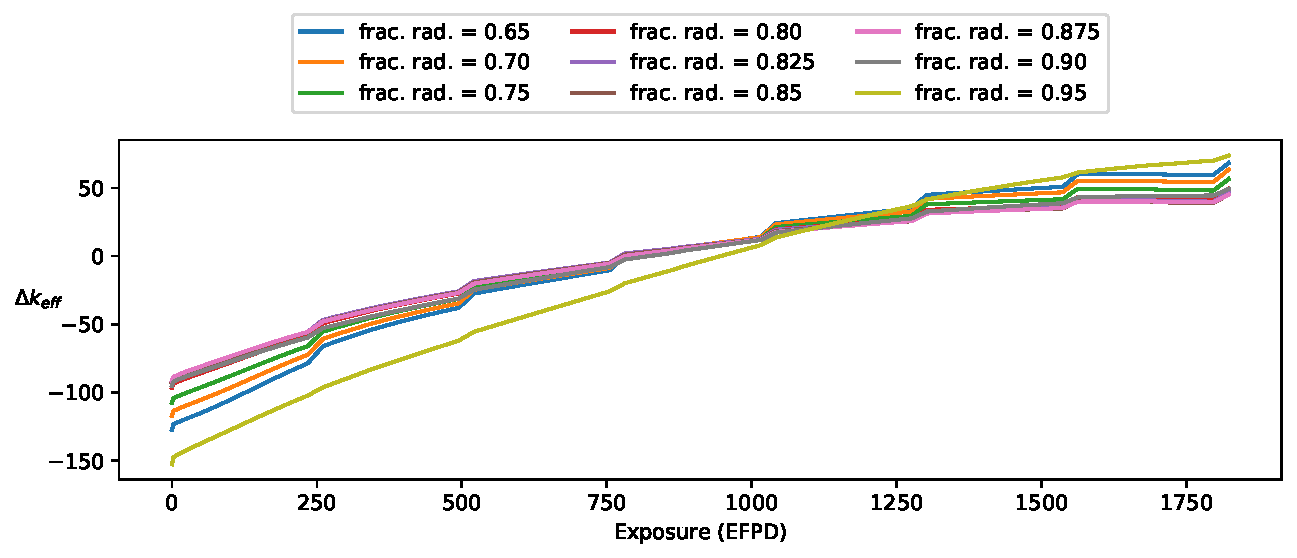
\includegraphics[width=\linewidth]{1a/FuelRadius-Eigenvalues}
            \caption{Eigenvalue comparisons for problem 1A using various inner fuel radii. \label{fig:LSMOC:1a:FuelRadius:Eigenvalue}}
        \end{figure}
        \begin{figure}
          \centering
          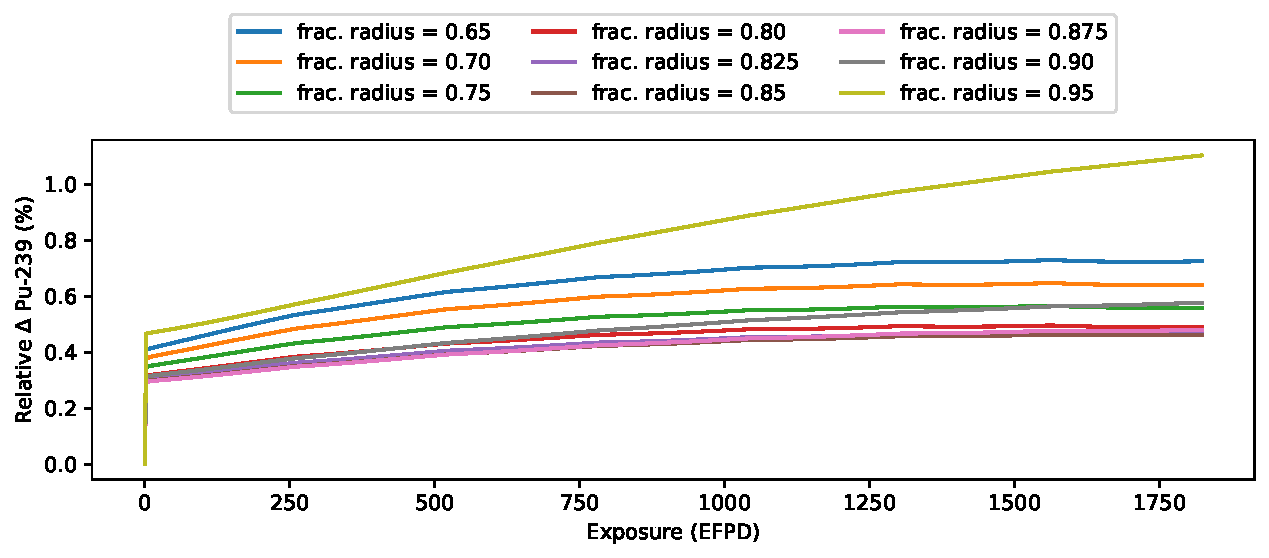
\includegraphics[width=\linewidth]{1a/FuelRadius-Pu239}
          \caption{Pu-239 concentration comparisons for problem 1A using various inner fuel radii. \label{fig:LSMOC:1a:FuelRadius:Pu239}}
        \end{figure}
      }
      \paragraph{Moderator Ring and Azimuthal Divisions} {
        The remaining mesh parameters are the azimuthal divisions in the fuel, clad, gap, and moderator regions, and the presence of an additional surrounding ring of moderator.
        While it may be sufficient to use a single azimuthal division in some regions in larger cases, due to symmetry of this single pin case, using a single azimuthal region would cause the linear components of the source to be zero (i.e. it is equivalent to the \ac{FSA}).
        It was found that the coarsening of these parameters have an insignificant affect on the resulting eigenvalue when using the \ac{LSA}, with less than 1 \ac{pcm} difference over the entire depletion.
        Thus, four azimuthal divisions in each material region, and no additional surrounding moderator ring was found to be sufficiently accurate in this case.
      }
      The coarse default and coarse meshes are displayed in \cref{figs:LSMOC:1A:Mesh}.

      \begin{figure}[h]
          \centering
          \begin{subfigure}[t]{0.45\textwidth}
              \centering
              
\includegraphics[width=0.9\textwidth]{1a/1a-default-trimmed}
              \caption{default mesh\label{fig:LSMOC:1a:Default Mesh}}
          \end{subfigure}%
          ~
          \begin{subfigure}[t]{0.45\textwidth}
              \centering
              
\includegraphics[width=0.9\textwidth]{1a/1a-coarse-trimmed}
              \caption{coarse mesh\label{fig:LSMOC:1a:Coarse Mesh}}
          \end{subfigure}
          \caption{VERA problem 1A (a) default and (b) coarse meshes.\label{figs:LSMOC:1A:Mesh}}
      \end{figure}
    }

    \subsection{VERA Problem 2A and 2P Depletion}{\label{ssec:LSMOC:VERA Problem 2A and 2P Depletion}
      A mesh study similar to that done in \cref{ssec:LSMOC:Typical Pin Cell Depletion} was performed on modified \ac{VERA} problems 2A and 2P \cite{VERAProblems} with isotopic depletion up to 70 \ac{GWDMT}.
      This was done to verify that the meshing parameters previously found were valid for larger problems, and determine if even coarser parameters were sufficient.
      First, problem 2A was studied; the meshing parameters of the fuel cell and guide-tube cells were studied independently.
      \subsubsection{Problem 2A}{\label{sssec:LSMOC:Problem 2A}
        \paragraph{2A - Default Mesh}{
          For this problem, a reference calculation was carried out on the lattice with a very fine mesh.
          This reference calclation also used a finer directional quadrature of 128 azimuthal angles and 4 polar angles, with a uniform ray-spacing of 0.001 cm.
          Again, the MPACT's current default mesh was used a starting point for the mesh study; the results of the \ac{FS} and \ac{LS} calculations on this default mesh are used as a baseline.
          Eigenvalue and pin-power comparisons are provided in \cref{fig:LSMOC:2A:Default Mesh:Eigenvalues,fig:LSMOC:2A:Default Mesh:PinPowers}.

          The trend in eigenvalue is similar to that found for problem 1A with the default mesh;
            the \ac{LS} calculation has a higher absolute eigenvalue difference of 51 \ac{pcm} compared to the \ac{FS} calculation with 43 \ac{pcm}.
          However, the average eigenvalue differences are similar at 24 and 21 \ac{pcm} for the \ac{FS} and \ac{LS} calculations, respectively.
          Additionally, \cref{fig:LSMOC:2A:Default Mesh:PinPowers} shows that maximum pin power differences are consistently lower for the linear source calculation.
          This indicates that local effects are predicted better by the linear source, and there is some cancellation of errors occurring in the eigenvalue.

          \begin{figure}
            \centering
            \includegraphics[width=\linewidth]{2a/DefaultMesh-Eigenvalues}
            \caption{VERA Problem 2A default mesh eigenvalue comparison. \label{fig:LSMOC:2A:Default Mesh:Eigenvalues}}
          \end{figure}
          \begin{figure}
            \centering
            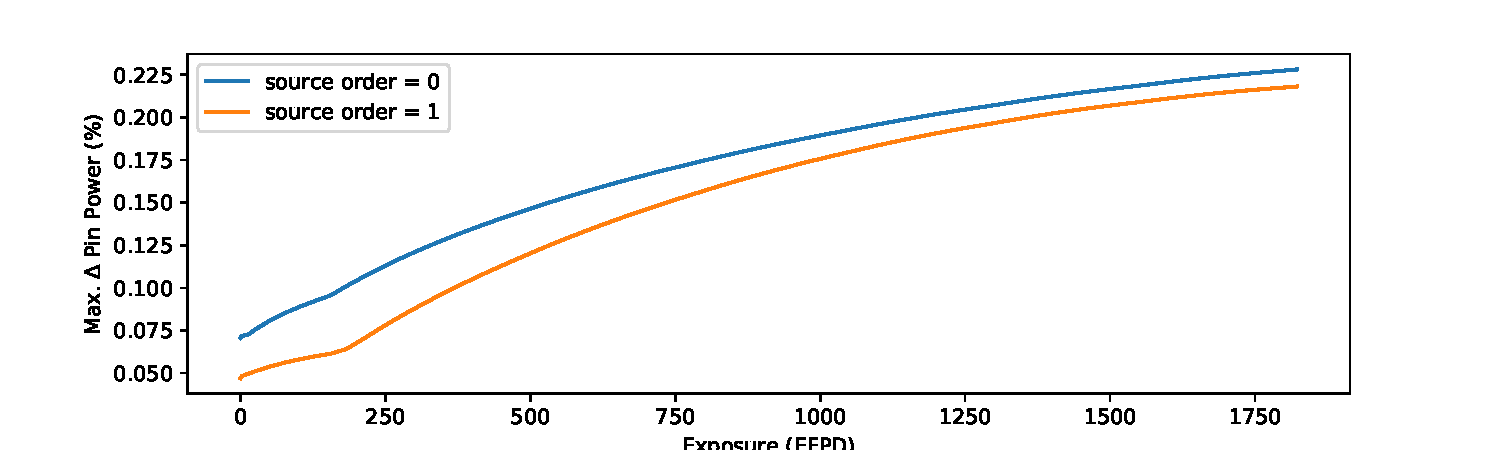
\includegraphics[width=\linewidth]{2a/DefaultMesh-PinPowers}
            \caption{VERA Problem 2A default mesh pin power comparison. \label{fig:LSMOC:2A:Default Mesh:PinPowers}}
          \end{figure}
        }
        \paragraph{2A - Fuel Radius and Azimuthal Divisions}{
          For this problem, only the fractional radius found in \cref{ssec:LSMOC:Typical Pin Cell Depletion} is tested against the current default mesh.
          There was no significant affect in eigenvalue or pin powers by using the 2-ring model with an inner radius fraction of 0.875.
          Next, the varied azimuthal divisions in the fuel were tested; this time testing a single azimuthal division.
          \Cref{fig:LSMOC:2A:Fuel Azimuthals:Eigenvalues} shows that there is noticeable affect moving to a single azimuthal division;
            however, the mean difference is changed by less than 1 \ac{pcm}, and the max difference is actually improved by 3 \ac{pcm}.
          We acknowledge that this improvement is likely due to cancellation of errors. Regardless, the net effect of this change is small.

          \begin{figure}
            \centering
            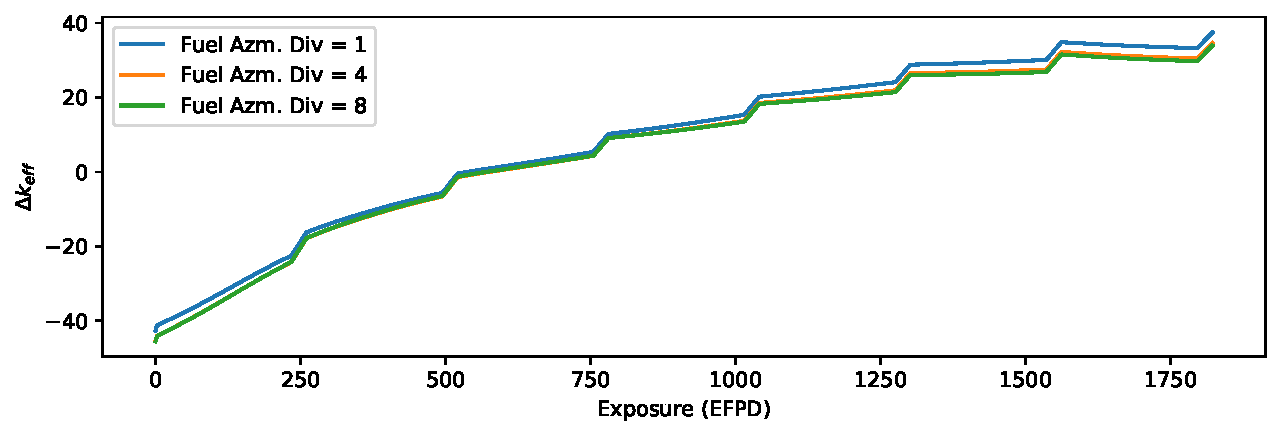
\includegraphics[width=\linewidth]{2a/FuelAzimuthals-Eigenvalue}
            \caption{VERA Problem 2A eigenvalue comparison for varied fuel azimuthal divisions. \label{fig:LSMOC:2A:Fuel Azimuthals:Eigenvalues}}
          \end{figure}
        }
        \paragraph{2A - Moderator Azimuthal Divisions}{
          The azimuthal divisions of the surrounding moderator seems to have a more significant effect on the accuracy of the calculation.
          As shown by \cref{fig:LSMOC:2A:Moderator Azimuthal:Eigenvalues}, using 4 azimuthal divisions seems to be sufficient; but moving to a single division is not feasible.
          A single division ore than doubles the mean eigenvalue difference, and shows a consistent positive bias.

          \begin{figure}
            \centering
            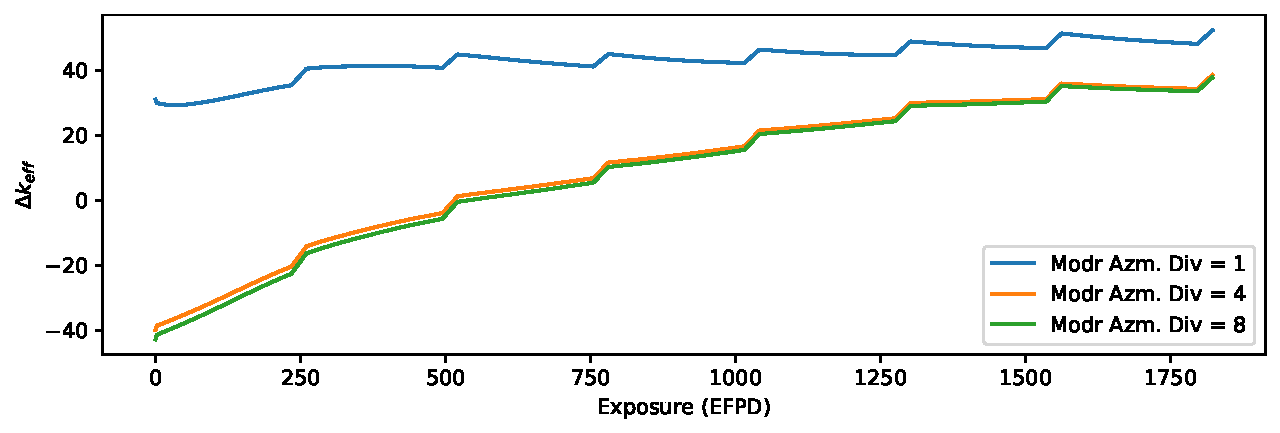
\includegraphics[width=\linewidth]{2a/ModrAzimuthals-Eigenvalue}
            \caption{VERA Problem 2A eigenvalue comparison for varied number of surrounding moderator azimuthal divisions in the fuel cells. \label{fig:LSMOC:2A:Moderator Azimuthal:Eigenvalues}}
          \end{figure}
        }
        \paragraph{2A - Cladding and Gap Azimuthal Divisions}{
          The azimuthal divisions of the cladding and gap regions do not seem to play a significant role.
          The difference is not even visually apparent in a graph of the eigenvalue, as seen in \cref{fig:LSMOC:2A:Clad Azimuthal:Eigenvalues}.

          \begin{figure}
            \centering
            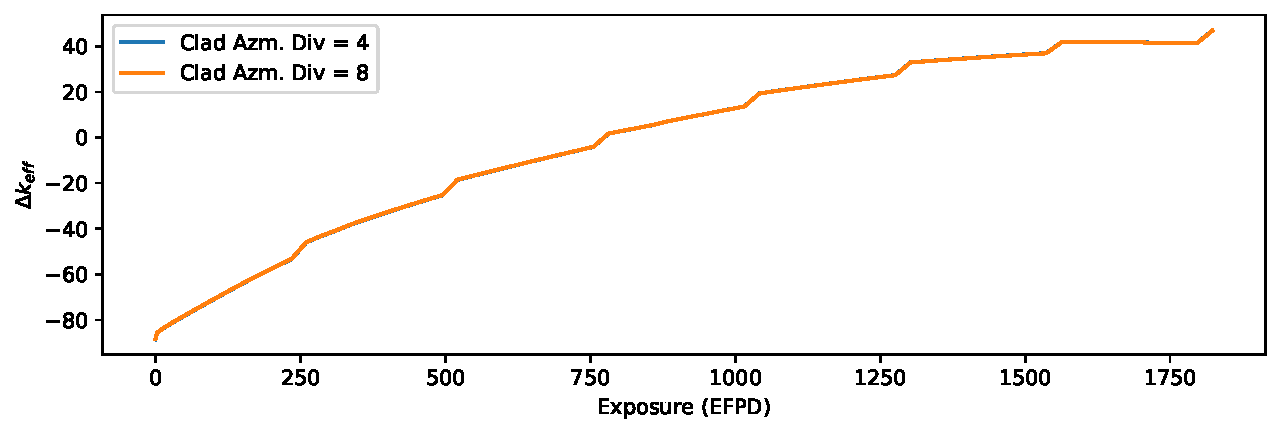
\includegraphics[width=\linewidth]{2a/CladAzimuthals-Eigenvalue}
            \caption{VERA Problem 2A eigenvalue comparison for varied number of the cladding/gap azimuthal divisions in the fuel cells. \label{fig:LSMOC:2A:Clad Azimuthal:Eigenvalues}}
          \end{figure}
        }
        \paragraph{2A - Guide-Tube Azimuthal Divisions}{
          In the 2A lattice, guide-tube pins are present; each guide-tube consists of three regions: inner moderator, cladding, and outer moderator.
          The effect of different azimuthal divisions in each of these regions was tested; the resulting eigenvalues are shown in \cref{fig:LSMOC:2A:Gtube:Inner Moderator Azimuthals:Eigenvalues,fig:LSMOC:2A:Gtube:Cladding Azimuthals:Eigenvalues,fig:LSMOC:2A:Gtube:Outer Moderator Azimuthals:Eigenvalues}.
          A single azimuthal division in each of these regions seems to be sufficient, without any significant affect on eigenvalue accuracy.
          However, 4 azimuthal divisions in the surrounding moderator was selected for moving forward due to compatibility issues with \ac{CTF}.

          \begin{figure}
            \centering
            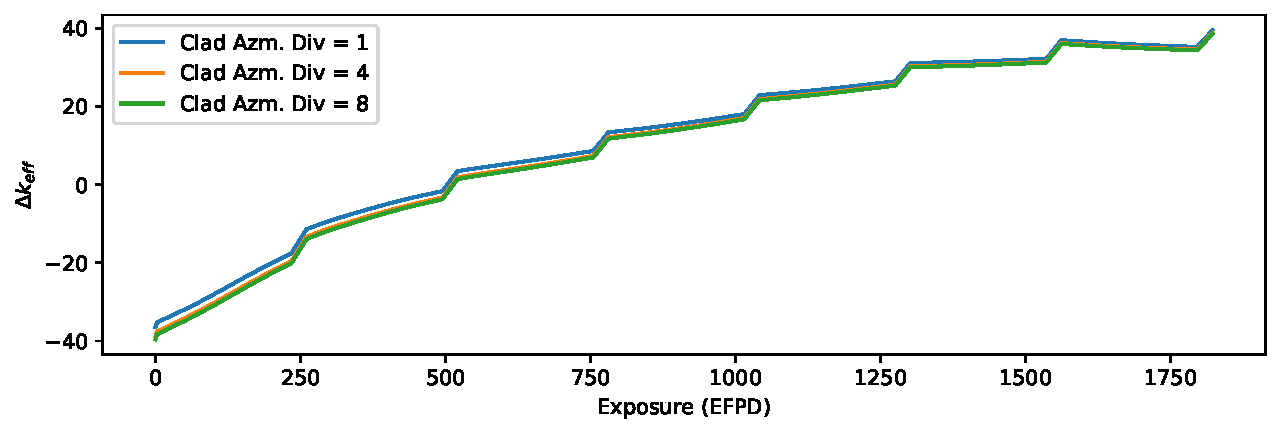
\includegraphics[width=\linewidth]{2a/Gtube-InnerModeratorAzm-Eigenvalue}
            \caption{VERA Problem 2A eigenvalue comparison for varied number of inner moderator azimuthal divisions in the guide-tube cells. \label{fig:LSMOC:2A:Gtube:Inner Moderator Azimuthals:Eigenvalues}}
          \end{figure}
          \begin{figure}
            \centering
            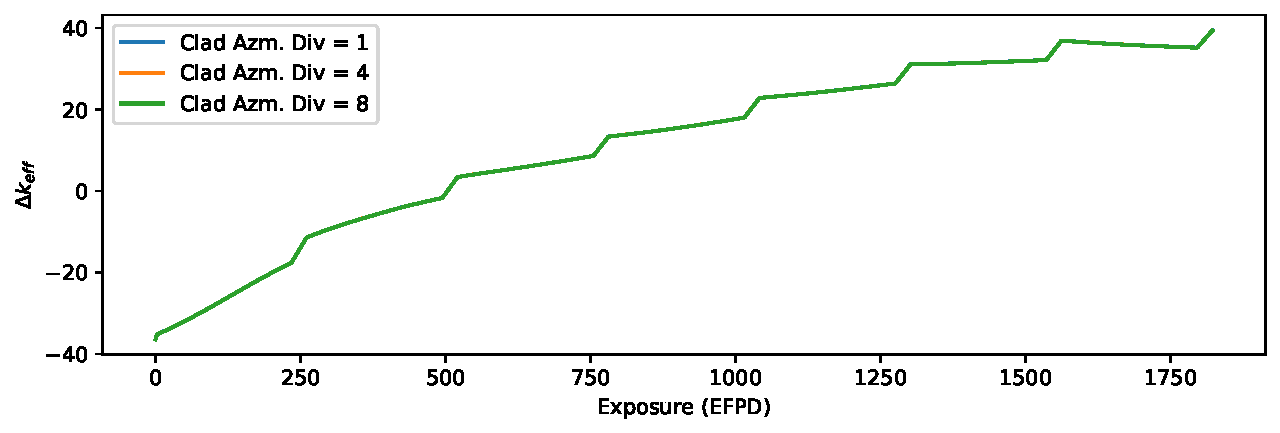
\includegraphics[width=\linewidth]{2a/Gtube-CladAzm-Eigenvalue}
            \caption{VERA Problem 2A eigenvalue comparison for varied number of cladding azimuthal divisions in the guide-tube cells. \label{fig:LSMOC:2A:Gtube:Cladding Azimuthals:Eigenvalues}}
          \end{figure}
          \begin{figure}
            \centering
            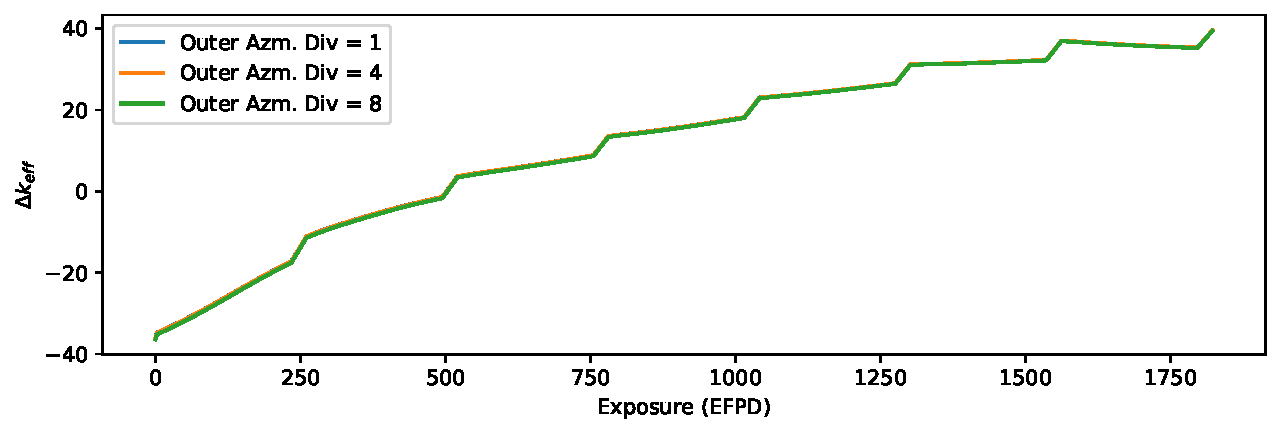
\includegraphics[width=\linewidth]{2a/Gtube-OuterAzm-Eigenvalue}
            \caption{VERA Problem 2A eigenvalue comparison for varied number of outer moderator azimuthal divisions in the guide-tube cells. \label{fig:LSMOC:2A:Gtube:Outer Moderator Azimuthals:Eigenvalues}}
          \end{figure}
        }
        \paragraph{2A - Coarse Mesh Summary}{
          Coarse mesh parameters were found using this isotopic depletion calculation on \ac{VERA} problem 2A.
          The fuel cell
          \begin{itemize}
            \item{has 2 fuel rings, with the inner radius being 0.875 fraction of the outer,}
            \item{no additional moderator ring in the surrounding moderator,}
            \item{a single azimuthal division in the fuel, clad, and gap regions,}
            \item{and four azimuthal divisions in the surrounding moderator.}
          \end{itemize}
          The guide-tube cell
          \begin{itemize}
            \item{has no additional moderator ring in the surrounding moderator,}
            \item{has a single azimuthal division for the inner moderator, and cladding,}
            \item{and four azimuthal divisions for the surrounding moderator.}
          \end{itemize}
          The lattice meshes are shown in \cref{figs:LSMOC:2a:Meshes}.

          \begin{figure}[h]
              \centering
              \begin{subfigure}[t]{0.45\textwidth}
                  \centering
                  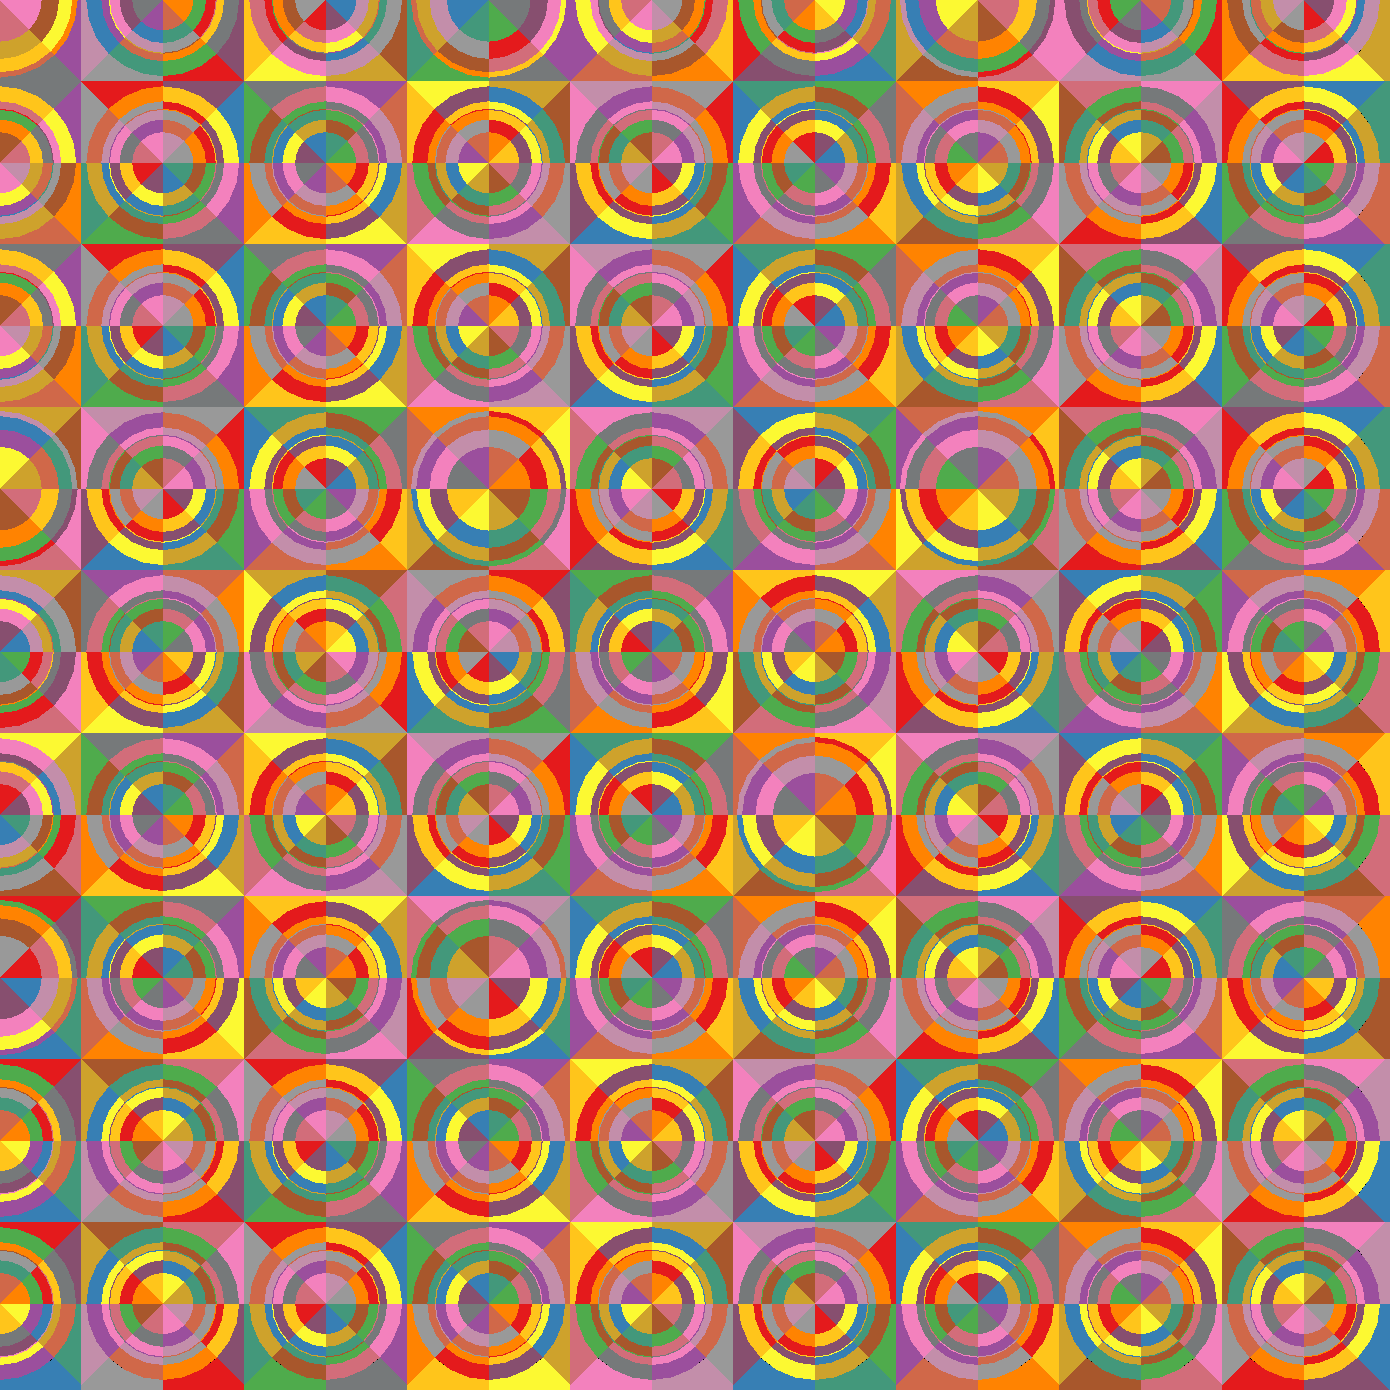
\includegraphics[width=0.9\textwidth]{2a/2a-default-trimmed}
                  \caption{default mesh\label{fig:LSMOC:2a:Default Mesh}}
              \end{subfigure}%
              ~
              \begin{subfigure}[t]{0.45\textwidth}
                  \centering
                  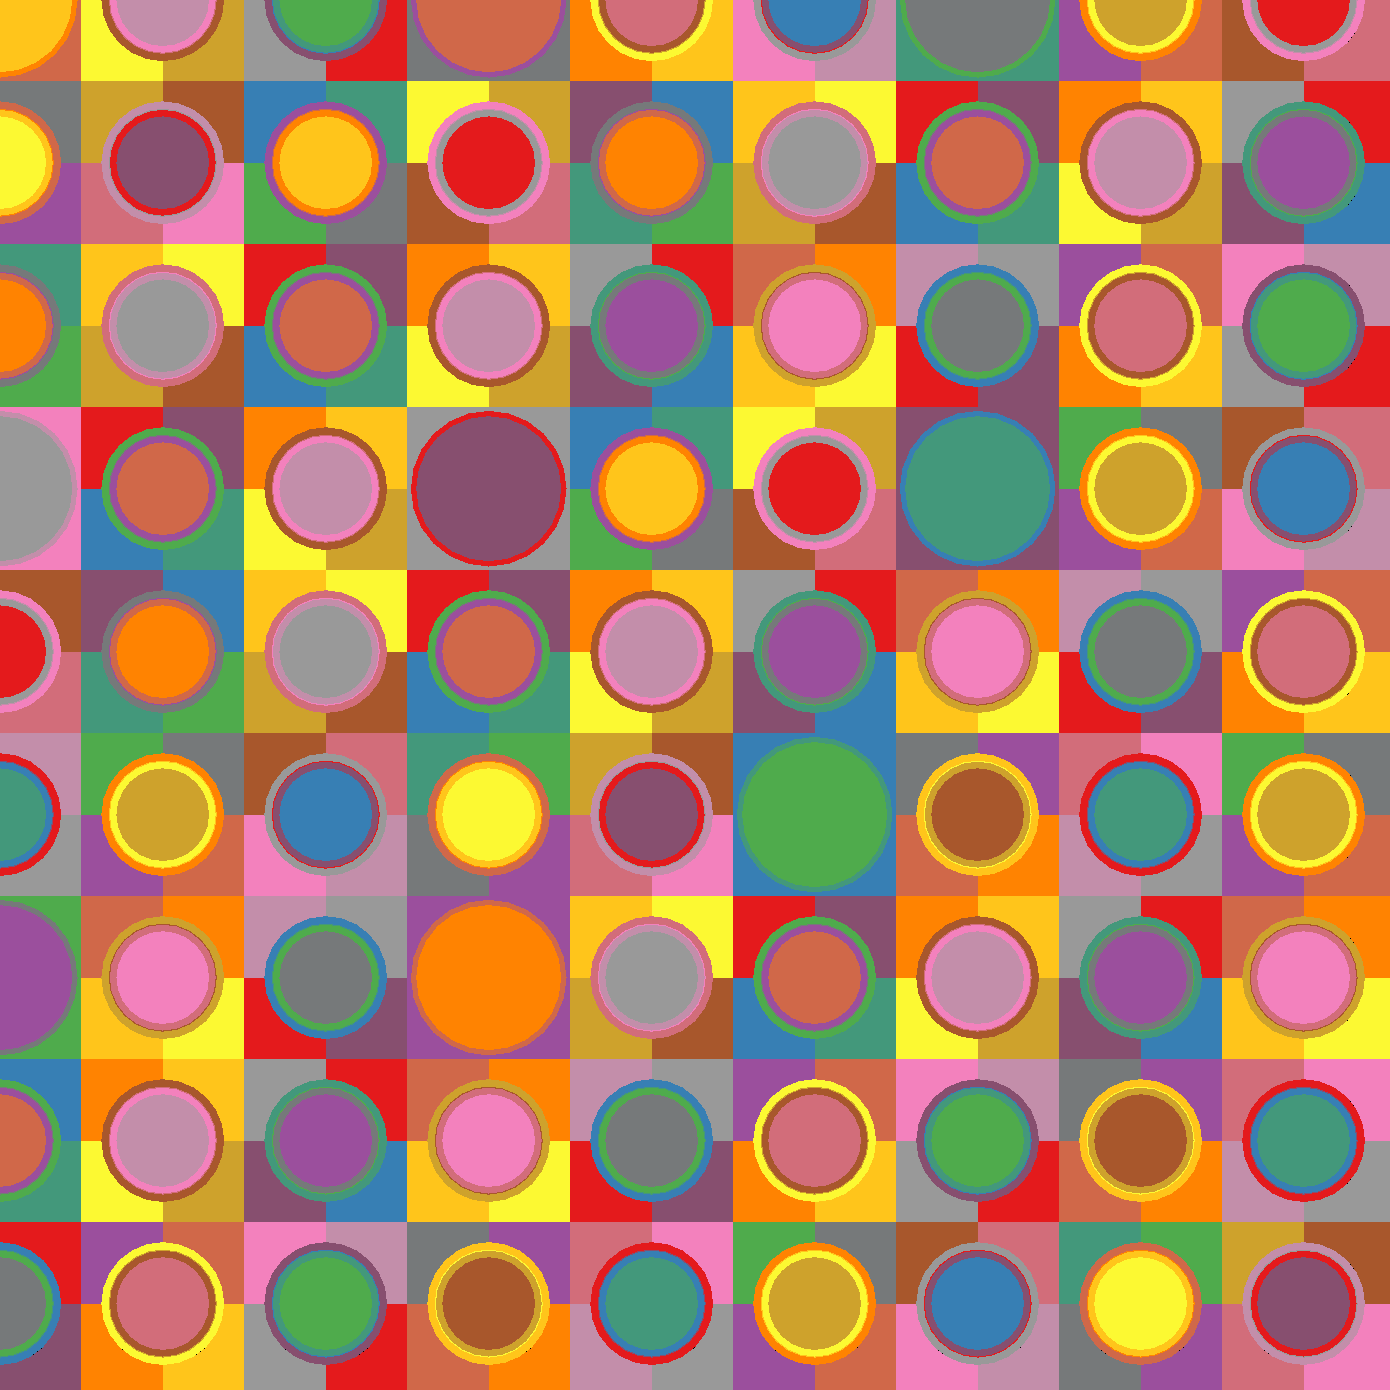
\includegraphics[width=0.9\textwidth]{2a/2a-coarse-trimmed}
                  \caption{coarse mesh\label{fig:LSMOC:2a:Coarse Mesh}}
              \end{subfigure}
              \caption{VERA problem 2A (a) default and (b) coarse meshes.\label{figs:LSMOC:2a:Meshes}}
          \end{figure}

          Eigenvalue comparisons are shown in \cref{fig:LSMOC:2A:Coarse Mesh:Eigenvalues}, and pin power comparisons are made in \cref{fig:LSMOC:2A:Coarse Mesh:PinPowers}.
          While it is visually apparent that the accuracy is made slightly worse than the default mesh \ac{LS} calculation, the entire goal of the this mesh study was to maintain error with the \ac{FS} calculation.
          This goal has been met, while reducing the number of cells from 3946 to 579.

          \begin{figure}
            \centering
            \includegraphics[width=\linewidth]{2a/Final-Eigenvalues}
            \caption{VERA Problem 2A coarse mesh eigenvalue comparison. \label{fig:LSMOC:2A:Coarse Mesh:Eigenvalues}}
          \end{figure}
          \begin{figure}
            \centering
            \includegraphics[width=\linewidth]{2a/Final-PinPowers}
            \caption{VERA Problem 2A coarse mesh pin power comparison. \label{fig:LSMOC:2A:Coarse Mesh:PinPowers}}
          \end{figure}
        }
      }

      \subsubsection{Problem 2P}{\label{sssec:LSMOC:Problem 2P}
        \paragraph{2P - Applying Coarse Mesh Parameters}{
          \ac{VERA} problem 2P contains several gadolinia enriched fuel rods; as the lattice is depleted, these fuel rods ``burn'' the gadolinia.
          The gadolinia is primarily burned away started at the outer radius and moving inwards as time progresses.
          This inward burning makes the pins difficult to model, and requires many radial divisions for accurate calculations; it is effectively a ``moving rim effect''.
          Additionally, because the presence of these small radial regions, a finer ray-spacing (0.01 cm) is necessary.

          To evaluate if the previously determined coarse mesh parameters are sufficient in this problem, they are applied to the regular fuel and guide-tube cells, while the gadolinia rods use the default meshing parameters.
          \Cref{fig:LSMOC:2P:Default Mesh:Eigenvalues,fig:LSMOC:2P:Default Mesh:PinPowers} show that applying the coarse mesh parameters to the fuel and guide-tube cells does not significantly worsen the eigenvalue or pin power results.
          It is worth observing that errors in this cases are significantly higher than in the problem 2A; this is likely due to the complicated radial dependence of the gadolinia rods during depletion.

          \begin{figure}
              \centering
              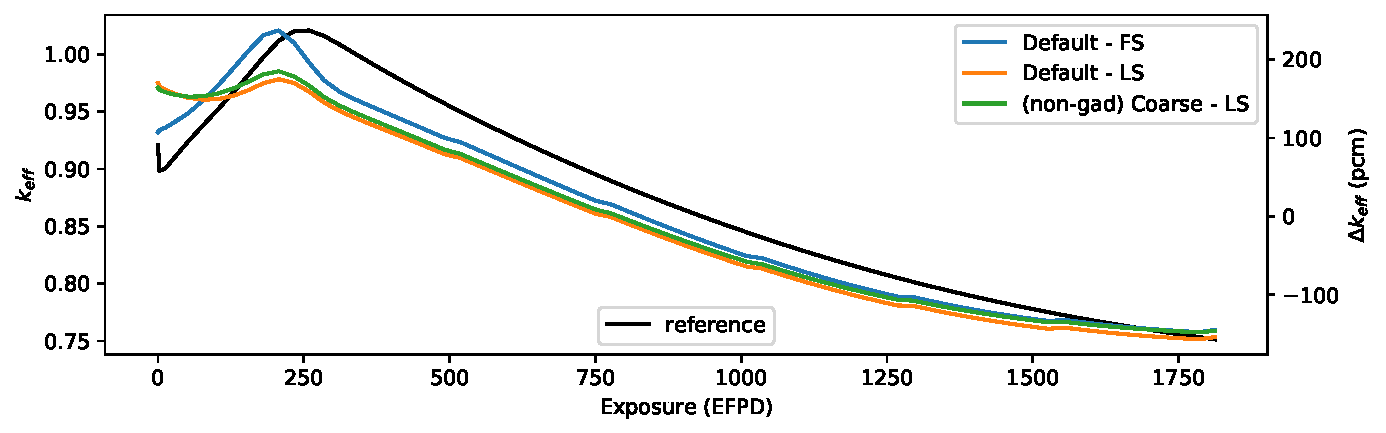
\includegraphics[width=\linewidth]{2p/Initial-Eigenvalues}
              \caption{Eigenvalue comparisons for VERA problem 2P with default mesh parameters and coarse mesh parameters for the fuel and guide-tube cells.\label{fig:LSMOC:2P:Default Mesh:Eigenvalues}}
          \end{figure}
          \begin{figure}
            \centering
            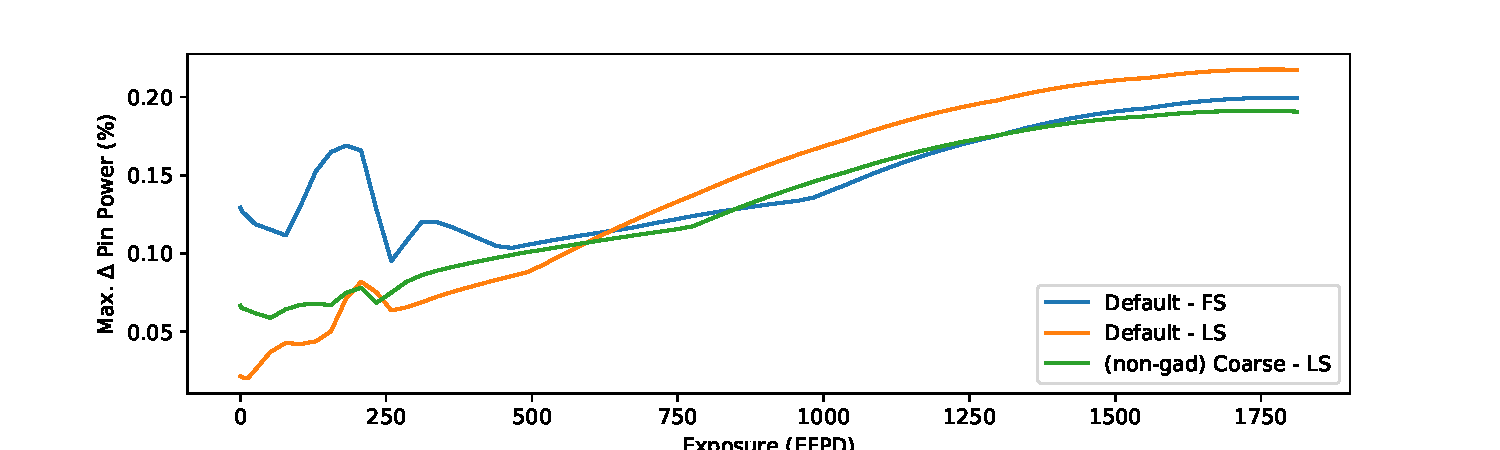
\includegraphics[width=\linewidth]{2p/Initial-PinPowers}
            \caption{Pin power comparisons for VERA problem 2P with default mesh parameters and coarse mesh parameters for the fuel and guide-tube cells.\label{fig:LSMOC:2P:Default Mesh:PinPowers}}
          \end{figure}
        }
        \paragraph{2P - Azimuthal Divisions}{
          It is not expected that the radial divisions in the gadolinia rods can be significantly coarsened.
          However, this is not true for the azimuthal divisions.
          We apply the same azimuthal divisions as we did for the fuel: 1 in the fuel, clad, and gap, and 4 in the surrounding moderator.
          \Cref{fig:LSMOC:2P:Gad Azm:Eigenvalues} shows the eigenvalue results are similar at all but the initial state to the previous coarse mesh parameters.
          Even at the initial state, the error is between the flat and linear source calculations on the default mesh.
          Thus, it is ``acceptable'' to coarsen the azimuthal divisions in the gadolinia pins.

          \begin{figure}
            \centering
            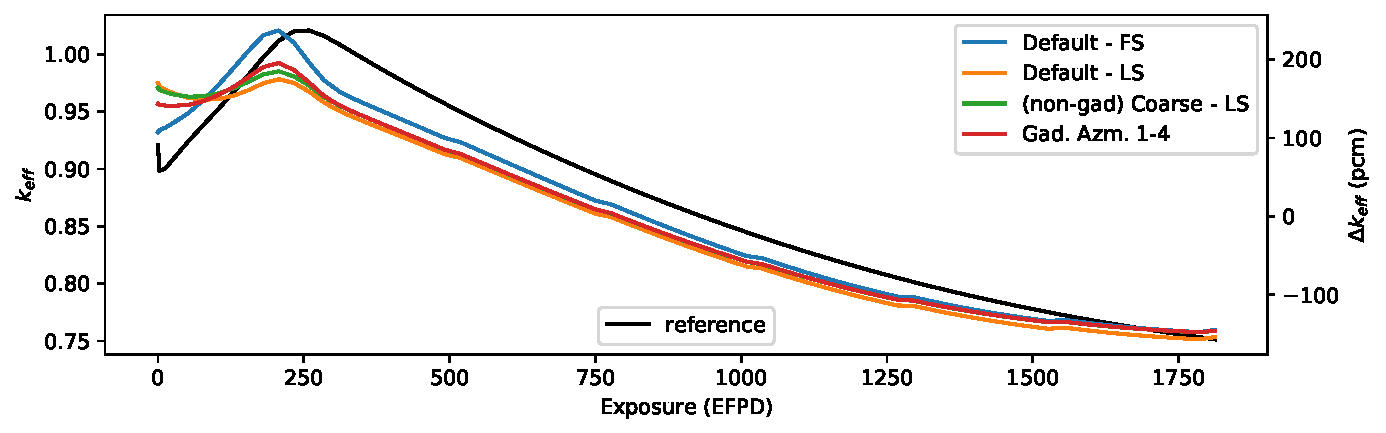
\includegraphics[width=\linewidth]{2p/GadAzm-Eigenvalues}
            \caption{Eigenvalue comparisons for VERA problem 2P for the default mesh, previous coarse mesh, and gadolinia rods with fewer azimuthal divisions.\label{fig:LSMOC:2P:Gad Azm:Eigenvalues}}
          \end{figure}
        }
        \paragraph{2P - Radial Divisions}{
          While it is unexpected that significant radial coarsening can occur in these pins, it is best to test this assumption.
          \Cref{fig:LSMOC:2P:Gad Rad:Eigenvalues} shows the eigenvalue errors for several different numbers of equal volume radii in the gadolinia fuel rods.
          It is clear that the number of radii can significantly affect the accuracy.
          For 8 radial divisions, the error is higher near the reactivity peak, it is still between the flat and linear source calculation errors on the default mesh.
          The goal of these mesh reduction studies was not to preserve the accuracy of the linear source on the default mesh, but to nearly match the accuracy of the flat source calculation on the default mesh.
          For this goal, 8 radial divisions seems to be sufficient.

          \begin{figure}
              \centering
              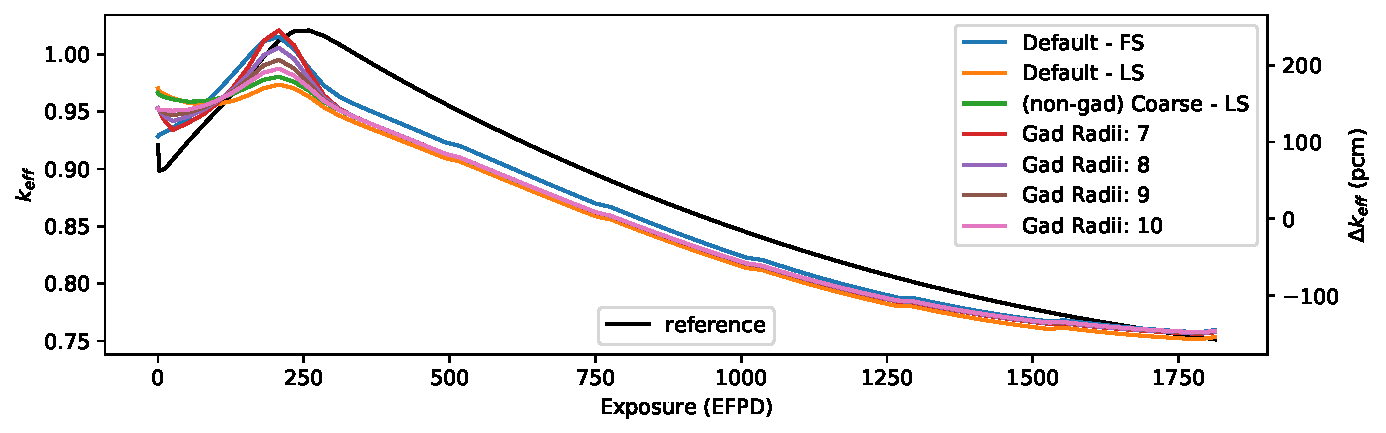
\includegraphics[width=\linewidth]{2p/GadRad-Eigenvalues}
              \caption{Eigenvalue comparisons for VERA problem 2P for varied number of radii in gadolinia rods.\label{fig:LSMOC:2P:Gad Rad:Eigenvalues}}
          \end{figure}
        }
        \paragraph{2P - Coarse Mesh Summary}{
          The coarse mesh parameters for the fuel and guide-tube cells previously found were also found to be sufficient for \ac{VERA} problem 2P.
          For the gadolinia rods, it was found to be sufficient to
          \begin{itemize}
            \item{have no additional moderator ring,}
            \item{use 8 equal volume fuel radial fuel divisions,}
            \item{a single azimuthal division in the fuel, clad, and gap regions,}
            \item{and four azimuthal divisions in the surrounding moderator.}
          \end{itemize}

          Eigenvalue comparisons are shown in \cref{fig:LSMOC:2P:Coarse Mesh:Eigenvalues}, and pin power comparisons are made in \cref{fig:LSMOC:2P:Coarse Mesh:PinPowers}.
          Using these coarse mesh parameters reduces the number of cells from 4282 to 621.
          The lattice meshes are visualized in \cref{figs:LSMOC:2p:Meshes}.

          \begin{figure}[h]
            \centering
            \begin{subfigure}[t]{0.45\textwidth}
                \centering
                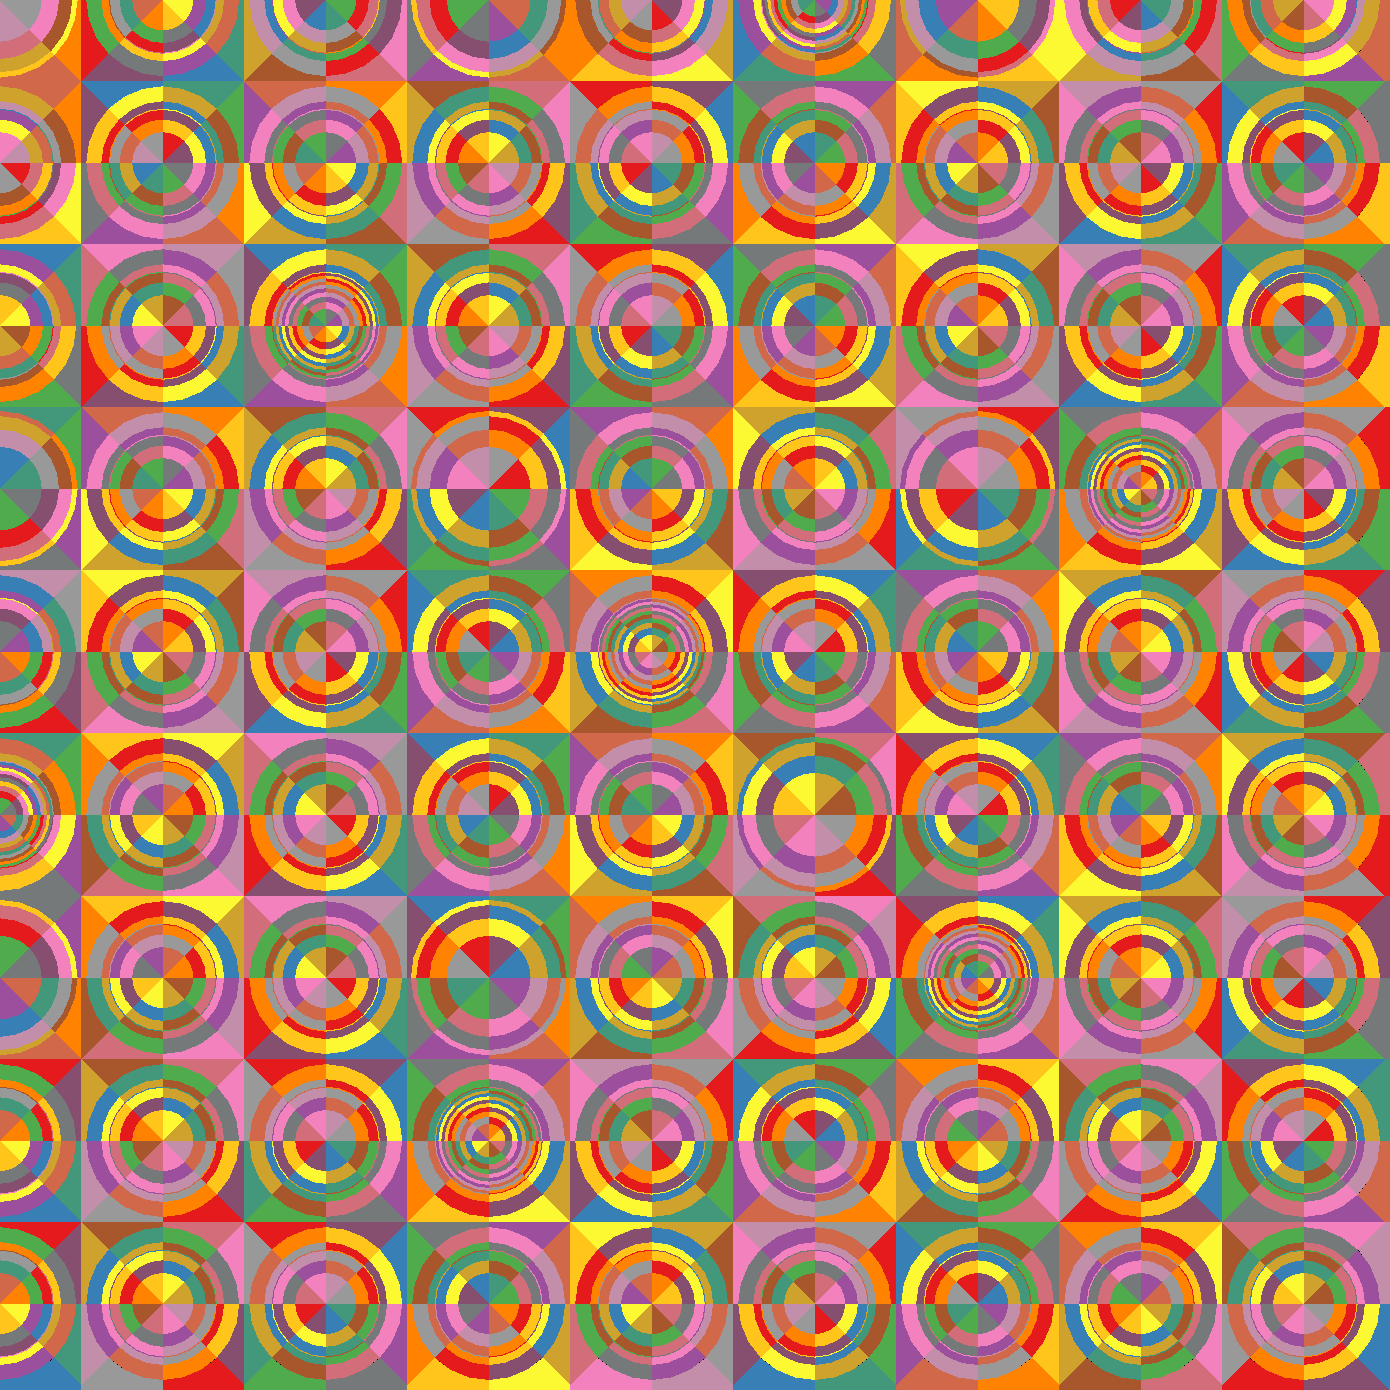
\includegraphics[width=0.9\textwidth]{2p/2p-default-trimmed}
                \caption{default mesh\label{fig:LSMOC:2p:Default Mesh}}
            \end{subfigure}%
            ~
            \begin{subfigure}[t]{0.45\textwidth}
                \centering
                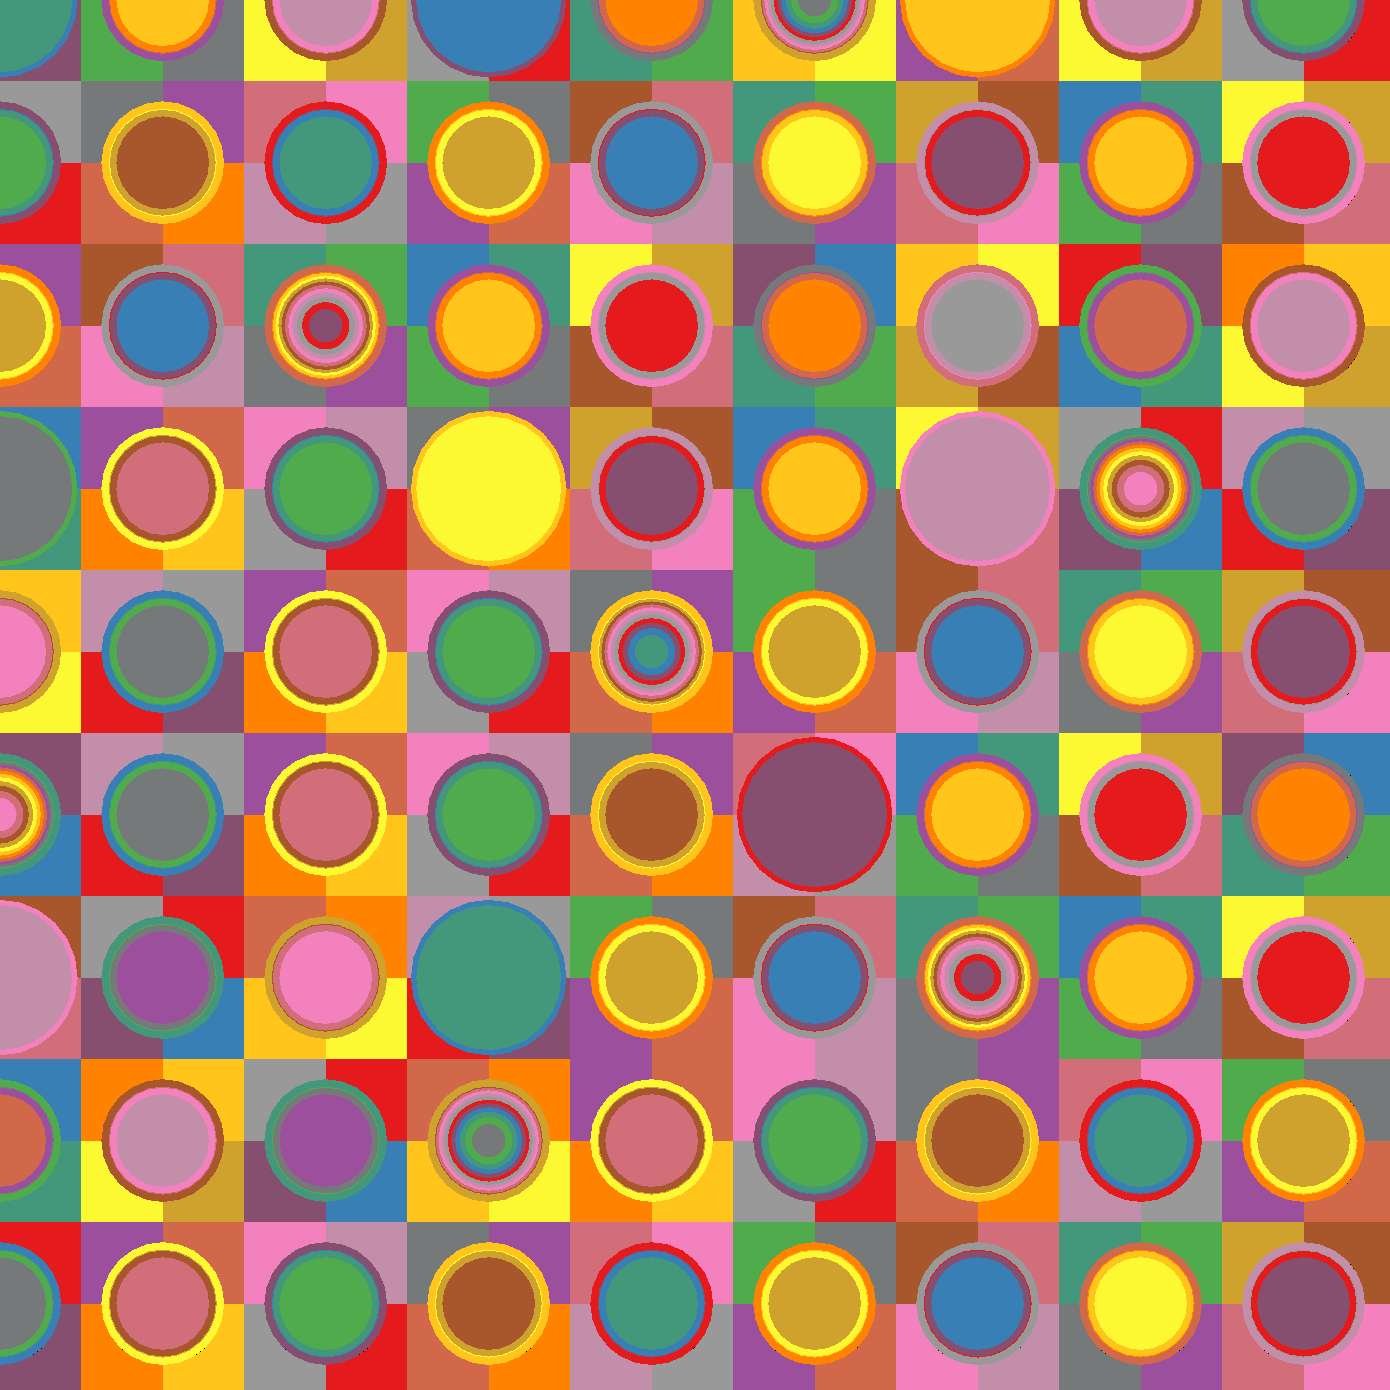
\includegraphics[width=0.9\textwidth]{2p/2p-coarse-trimmed}
                \caption{coarse mesh\label{fig:LSMOC:2p:Coarse Mesh}}
            \end{subfigure}
            \caption{VERA problem 2P (a) default and (b) coarse meshes.\label{figs:LSMOC:2p:Meshes}}
          \end{figure}

          \begin{figure}
            \centering
            \includegraphics[width=\linewidth]{2p/Final-Eigenvalues}
            \caption{VERA Problem 2P coarse mesh eigenvalue comparison. \label{fig:LSMOC:2P:Coarse Mesh:Eigenvalues}}
          \end{figure}
          \begin{figure}
            \centering
            \includegraphics[width=\linewidth]{2p/Final-PinPowers}
            \caption{VERA Problem 2P coarse mesh pin power comparison. \label{fig:LSMOC:2P:Coarse Mesh:PinPowers}}
          \end{figure}
        }
      }

      \subsubsection{Performance}{\label{sssec:Performance}
        [TIME/MEMORY RESULTS HERE]
      }
    }

    \subsection{2-D Lattices}{\label{ssec:LSMOC:2-D Lattices}
      In order to evaluate these coarse mesh parameters, they were applied to the \ac{VERA} problem 2 lattice series.
      This series contains 17 common lattice configurations, and it is expected that if the meshing parameters are sufficient for these cases, they will be sufficient in most applications.
      The eigenvalue and pin-power results compared to a very finely meshed reference case are shown in \cref{tab:LSMOC:Lattice Results}.
      On average, the \ac{LS} on the coarse mesh, using the parameters found in the previous sections, had accuracy comparable to the \ac{FS} on the default mesh.
      Additionally, the worst case errors were lower for the \ac{LS} on the coarse mesh.
      These results also show that the \ac{FS} on the coarse mesh is not sufficient, with significantly worse eigenvalue and pin-power comparisons.

      \begin{table}
        \centering
        \caption{Results for VERA Problem 2 lattices for different mesh and source approximations.}
        \footnotesize
        \begin{tabular}{rrrrr@{\hskip 1cm}rrrr} \toprule
          Case  & \multicolumn{4}{c}{$\Delta \keff$ (pcm)} & \multicolumn{4}{c}{Max Pin Power Difference (\%)}\\\midrule
                & FS Default & LS Default & FS Coarse & LS Coarse & FS Default & LS Default & FS Coarse & LS Coarse\\\midrule
                A    & -17  &   -51   &  44     & -36             & 0.07 & 0.05 & 0.24 & 0.08\\
                B    & -15  &   -49   &  46     & -34             & 0.07 & 0.05 & 0.24 & 0.08\\
                C    & -17  &   -51   &  44     & -36             & 0.07 & 0.05 & 0.24 & 0.08\\
                D    & -25  &   -59   &  39     & -41             & 0.07 & 0.05 & 0.24 & 0.08\\
                E    & -49  &   -40   &  -52    & -27             & 0.12 & 0.05 & 0.37 & 0.08\\
                F    & -74  &   -32   &  -120   & -26             & 0.15 & 0.05 & 0.51 & 0.08\\
                G    & -98  &   -45   &  -210   & -43             & 0.19 & 0.09 & 0.59 & 0.10\\
                H    & -78  &   17    &  -206   & 18              & 0.25 & 0.15 & 0.58 & 0.15\\
                I    & 2    &   -43   &  82     & -24             & 0.09 & 0.05 & 0.29 & 0.08\\
                J    & -74  &   -32   &  -119   & -26             & 0.10 & 0.05 & 0.34 & 0.08\\
                K    & -61  &   -26   &  -97    & -19             & 0.17 & 0.06 & 0.55 & 0.08\\
                L    & 60   &   37    &  105    & 52              & 0.13 & 0.07 & 0.35 & 0.12\\
                M    & 74   &   54    &  124    & 71              & 0.11 & 0.06 & 0.26 & 0.11\\
                N    & -1   &   31    &  -45    & 43              & 0.18 & 0.05 & 0.51 & 0.11\\
                O    & -21  &   9     &  -109   & 7               & 0.15 & 0.06 & 0.43 & 0.08\\
                P    & -115 &   -42   &  -311   & -64             & 0.17 & 0.08 & 0.69 & 0.14\\
                Q    & -12  &   -48   &  54     & -30             & 0.08 & 0.05 & 0.28 & 0.08\\\midrule
                AVG  & 47   &   39    &  106    & 35              & 0.13 & 0.06 & 0.39 & 0.09\\
                MAX  & 115  &   59    &  311    & 71              & 0.25 & 0.15 & 0.69 & 0.15\\\bottomrule
        \end{tabular}
        \label{tab:LSMOC:Lattice Results}
      \end{table}

      [ADD TABLE OF TIME (per iter?) / MEMORY][MAKE NOTE OF ITERATION NUMBERS]

      \subsubsection{Coarse Rays}{\label{sssec:LSMOC:Coarse Rays}
        In each of the these lattice calculations, the \ac{MOC} calculation takes up the majority of the runtime.
        The \ac{MOC} runtime is directly proportional to the number of track-segments that are generated during the ray-tracing.
        This number is reduced as the mesh becomes coarser; however, due to material and geometric limitations, the mesh can only be coarsened so much.
        Another parameter that affects the number of track-segments is the ray-spacing, or how far apart each ray is.
        The rays can be spaced more coarsely, but this may cause some regions to not be integrated as accurately, thus degrading overall accuracy.

        In this section, the use of coarser ray-spacing is investigated for the \ac{VERA} problem 2 series.
        Results were generated using a ray-spacing of 0.1 cm and 0.2 cm for the default mesh with the \ac{FS} solver, and for the coarse mesh with \ac{LS} solver.
        Eigenvalue and pin power comparisons are shown in \cref{tab:LSMOC:Lattice Results:Coarse Rays}.

        [SHOW DIFFERENCE FROM PREVIOUS!? - i.e. show affect of ray-spacing]

        [Coarse rays work well if there are no finely meshed elements!]

        \begin{table}
          \centering
          \caption{Results for VERA Problem 2 lattices for different mesh and source approximations and coarse ray-spacings.}
          \footnotesize
          \begin{tabular}{rrrrr@{\hskip 1cm}rrrr} \toprule
            Case  & \multicolumn{4}{c}{$\Delta \keff$ (pcm)} & \multicolumn{4}{c}{Max Pin Power Difference (\%)}\\\midrule
                  & FS (0.1 cm) & FS (0.2 cm) & LS (0.1 cm) & LS (0.2cm) & FS (0.1 cm) & FS (0.2 cm) & LS (0.1 cm) & LS (0.2cm)\\\midrule
            A     & 42   &   34    &  21   &   18   & 0.15 & 0.45 & 0.10 & 0.33\\
            B     & 41   &   33    &  19   &   16   & 0.15 & 0.45 & 0.10 & 0.33\\
            C     & 42   &   34    &  21   &   18   & 0.15 & 0.45 & 0.10 & 0.33\\
            D     & 45   &   38    &  23   &   20   & 0.15 & 0.45 & 0.10 & 0.33\\
            E     & 4    &   -59   &  25   &   -29  & 0.22 & 0.28 & 0.09 & 0.28\\
            F     & -22  &   -32   &  26   &   28   & 0.19 & 0.31 & 0.09 & 0.42\\
            G     & 27   &   73    &  98   &   162  & 0.31 & 0.49 & 0.24 & 0.44\\
            H     & -37  &   71    &  59   &   180  & 0.35 & 0.52 & 0.24 & 0.51\\
            I     & 54   &   45    &  25   &   22   & 0.16 & 0.47 & 0.10 & 0.32\\
            J     & -22  &   -31   &  26   &   28   & 0.19 & 0.31 & 0.08 & 0.42\\
            K     & -5   &   -15   &  37   &   38   & 0.20 & 0.33 & 0.10 & 0.43\\
            L     & -30  &   -171  &  70   &   -40  & 0.79 & 0.90 & 0.80 & 1.30\\
            M     & -140 &   -220  &  -43  &   -15  & 1.08 & 0.94 & 1.11 & 1.20\\
            N     & -95  &   -227  &  23   &   -103 & 0.91 & 0.85 & 0.98 & 0.98\\
            O     & 4    &   -36   &  27   &   -21  & 0.25 & 0.62 & 0.14 & 0.43\\
            P     & -7   &   -35   &  39   &   -7   & 0.30 & 0.61 & 0.20 & 0.40\\
            Q     & 43   &   35    &  22   &   19   & 0.15 & 0.46 & 0.11 & 0.32\\\midrule
            AVG   & 39   &   70    &  36   &   45   & 0.34 & 0.52 & 0.28 & 0.52\\
            MAX   & 140  &   227   &  98   &   180  & 1.08 & 0.94 & 1.11 & 1.30\\\bottomrule
          \end{tabular}
          \label{tab:LSMOC:Lattice Results:Coarse Rays}
        \end{table}
      }
    }

    \subsection{Assembly with Feedback}{\label{ssec:LSMOC:Assembly with Feedback}
      \ac{VERA} problem 6 is a single 3-D \ac{PWR} assembly with \ac{TH} feedback \cite{VERAProblems}.
      The coarse meshing parameters from the previous sections were applied to this problem;
        these results will help to determine whether or not the coarse mesh parameters are also sufficient when \ac{TH} feedback is present.
      As a 3-D assembly, this problem has lower and upper plates, and nozzles.
      These elements were models as rectilinear grids of 0.42$\times$0.42 cm$^2$ sized cells.

      This problem was run with the default and coarse meshes using the \ac{FSA} and \ac{LSA} solvers.
      A parallel spatial decomposition was applied into 58 sub-domains, each consisting of a single axial plane.
      Each case was compared against a very finely meshed case run using the \ac{LSA} solver.
      Each case used a Tabuchi-Yamamoto quadrature with 64 azimuthal angles and 4 polar angles, with a uniform ray-spacing of 0.05 cm.
      An additional case was run using the coarse mesh, \ac{LSA} solver, and 0.1 cm ray-spacing.

      Results are summarized in \cref{tab:LSMOC:P6:Results}, and performance metrics are listed in \cref{tab:LSMOC:P6:Performance}.
      It is quite clear that the \ac{LSA} solver on the coarse mesh is at least as accurate, for this problem, as the \ac{FSA} on the default mesh.
      Additionally, the \ac{FSA} on the coarse mesh performs significantly worse in every metric of \cref{tab:LSMOC:P6:Results}.
      Finally, it was shown that for this problem the use of coarser ray-spacing was possible and had very little affect on the results.
      Problem 6 has no inserted control rods or other finely meshed elements, and this is likely why using coarsely spaced rays is possible in this case.

      \Cref{tab:LSMOC:P6:Performance} might seem to imply that the \ac{LSA} solvers outperformed the \ac{FSA} solvers on the same mesh.
      This is not the case, as the \ac{LSA} cases required fewer iterations to converge.
      The iterations may differ due to non-uniform iterative convergence \footnote{due to complex eigenvalues in the spectral radius} that has previously been observed in problems with \ac{CMFD} acceleration and feedback \cite{Kochunas2017}.
      If the \ac{MOC} run-time per iteration is compared, the \ac{LSA} solver takes 79\% longer than the \ac{FSA} solver on the default mesh, but only 35\% longer on the coarse mesh.

      Because \ac{CTF} takes far longer in the first several iterations, it is not fair to compare total run-time per iteration.
      Rather, we can look at the time that the \ac{FSA} solver cases took to complete the same number of iterations the \ac{LSA} solver cases needed.
      The time to complete 9 iterations are shown in \cref{tab:LSMOC:P6:Performance}.
      These results still show that the use of the \ac{LSA} on the coarse mesh is advantageous compared to the default mesh with \ac{FSA}.
      The coarse mesh \ac{LSA} case reduced the run-time for 9 iterations by 4.8\%, but reduced \ac{MOC} run-time per iteration by 9.3\%.
      By also using coarse rays the run-time is reduced by 8.4\% for total time, and 72.7\% for \ac{MOC} time per iteration.

      The reduction in memory usage from using a coarser mesh is also an important aspect of the \ac{LSA} solvers.
      The coarse mesh \ac{LSA} case reduced total memory usage, compared to the default mesh \ac{FSA} case, by 15.5\%, and maximum process memory usage by 4.2\%.
      By using coarser ray-spacing, the reduction in total memory is significantly higher at 33.6\%, and 20.8\% reduction in maximum process memory.

      \begin{table}[htbp]
        \centering
        \caption{
          Results for VERA problem 6 simulations using different source approximations and mesh parameters.
          MPPE is the maximum pin-power error, and MPT is the maximum pin temperature.}
        \label{tab:LSMOC:P6:Results}
        \begin{tabular}{rrrrr}\toprule
          Solver & Mesh (Ray-Spacing) & $\Delta\keff$ (pcm) & MPPE (\%) & $\Delta$ MPT (K)\\\midrule
          FSA    & Default (0.05 cm)  & 34    & 0.31 & -0.9\\
          LSA    & Default (0.05 cm)  & -7    & 0.08 & -0.3\\
          FSA    & Coarse  (0.05 cm)  & 109   & 0.85 & -3.5\\
          LSA    & Coarse  (0.05 cm)  & 13    & 0.09 &  0.0\\
          LSA    & Coarse  (0.10 cm)  & 12    & 0.17 &  0.1\\\bottomrule
        \end{tabular}
      \end{table}

      \begin{table}[htbp]
        \centering
        \caption{
          Performance metrics for VERA problem 6 using different source approximations and mesh parameters.
        }
        \label{tab:LSMOC:P6:Performance}
        \begin{tabular}{rrrrrrrrrr}\toprule
                 &                    &            & \phantom{aa}& \multicolumn{3}{c}{Run-time (s)} & \phantom{aa} &\multicolumn{2}{c}{Memory (MB)}\\\cline{5-7}\cline{9-10}
          Solver & Mesh (Ray-Spacing) & Iterations && Total & 9 Iter. & MoC  && Total & Max.\\\midrule
          FSA    & Default (0.05 cm)  & 11         && 391 & 393 & 16.1 && 12438 & 264\\
          LSA    & Default (0.05 cm)  &  9         && 390 & 399 & 23.6 && 13156 & 272\\
          FSA    & Coarse  (0.05 cm)  & 11         && 379 & 379 & 10.8 && 10381 & 248\\
          LSA    & Coarse  (0.05 cm)  &  9         && 366 & 374 & 14.6 && 10506 & 253\\
          LSA    & Coarse  (0.10 cm)  &  9         && 354 & 360 &  4.4 &&  7887 & 209\\\bottomrule
        \end{tabular}
      \end{table}

      [INSERT VERAVIEW Pin-Power comparison for Default mesh FSA and Coarse mesh LSA]
    }

    \subsection{Core Depletion with Feedback}{\label{ssec:LSMOC:Core Depletion with Feedback}
      [Rough outline:
        1. P9 depletion and TH Feedback
        2. Radial coupling affect?
        3. Mesh is valid or no? w/o radial coupling? w/ radial coupling?
        4. Mention coarse rays = NO because control rods
      ]
    }
  }
  \section{Conclusions}{\label{sec:Conclusions}
    [INSERT CONCLUSIONS HERE]
  }

  % References
  \printbibliography
}